  % % GitHub cvitanov/reducesymm/tingnan/blog.tex   pdflatex blog
                        %% logical setup, no need to edit %%%%%%%%%%
                        \newif\ifpaper \newif\ifPDF               %%
                        \newif\ifOUP \newif\ifboyscout            %%
                        \newif\ifdasbuch                          %%
                        \newif\ifsolutions                        %%
                        \dasbuchfalse %% not DasBuch, not QFT lectures %%
                        \boyscouttrue %% commented, WWW/boyscouts %%
                        \solutionstrue %% include solutions       %%
                        \paperfalse\PDFtrue %% hyperlinked        %%
                        \OUPfalse                %% ChaosBook %%%%%%
    % Toggle between draft and non-draft versions
%\boyscoutfalse                 % public, for hyperlinked ChaosBook/projects
    % Toggle between draft and non-draft
%\articletrue                   %editing the article (May 2012: nonesuch)
%\articletrue\boyscoutfalse     % article for submission

% Predrag 2013-02-17 search for "uncomment" to make Gable parts visible
%                    transfer chaosbook/soluMaps toCB: Gable's solutions

\documentclass[10pt,openany]{book}
\usepackage{amsmath,amsfonts,amssymb}
\usepackage[nooneline]{caption} % Grigo figures?
\usepackage{color}
\usepackage{url}
\usepackage{fancyhdr}
\usepackage{alltt}
\usepackage{ifthen}
\usepackage{bm}
\usepackage[latin1]{inputenc}
\usepackage[T1]{fontenc}
\usepackage{times}
\usepackage[pdftex]{graphicx}
\usepackage{array}
\providecommand\phantomsection{} % with this it works without hyperref as well
\usepackage{verbatim}
%% inputs/layout.tex
% $Author$ $Date$

% from ChaosBook                        Predrag          5jun2008

\newcommand{\authorSFPC}[1] % Date 6 Jun 2009, for example
     {\hfill (S. Froehlich and P. Cvitanovi\'c, #1)}
\newcommand{\authorSF}[1]
     {\hfill (S. Froehlich, #1)}
\newcommand{\authorRW}[1]
     {\hfill (R. Wilczek, #1)}
\newcommand{\authorES}[1]
     {\hfill (E. Siminos, #1)}
\newcommand{\authorPC}[1]
     {\hfill (P. Cvitanovi\'c, #1)}


%%%%%%%% for figure layouts:
%% fine tuning floatingfigure \usepackage[nooneline] captions %%%%%
%        \renewcommand{\captionfont}{\footnotesize} % \sffamily}
%        \renewcommand{\captionlabelfont}{\footnotesize \bfseries \rmfamily}
%        % \renewcommand{\captionlabeldelim}{.\quad}
%        % \setlength{\captionmargin}{10pt}

% \FIG{#1}    % \includegraphics[width=0.40\textwidth]{Fig/f_name.ps}  ...
%     {#2}    % short caption text omitted here
%     {#3}    % full caption text
%     {#4}    % f-figure-label
\newcommand{\FIG}[4]{\begin{widefigure}[t]{#4}
    \widefigparts{\begin{minipage}[b]{0.98\textwidth}
                    #1\end{minipage}}{#3}\end{widefigure}}

\newcommand{\FFIG}[5]{\begin{floatingfigure}[v]{0.40\textwidth}
                      \noindent
                      \includegraphics[#1]{#2}
                      \caption[#3]{#4}
                      \label{#5}
              \end{floatingfigure} }

%   \BFIG{#1}   % width=#1\textwidth
%        {#2}   % f_name.ps
%    {#3}   % short caption text
%    {#4}   % full caption text
%    {#5}   % f-figure-label
%       defined here:
\newcommand{\BFIG}[5]{\begin{figure}
              \hspace*{0.10\textwidth}%
              \begin{minipage}[b]{1.00\textwidth}
              \centering{
                      \includegraphics[width=#1\textwidth]{Fig/#2}
                     }
                      \caption[#3]{#4}
                      \label{#5}
              \end{minipage}
              \end{figure} }

%  \SFIG{#1}    % f_name.png (or .pdf)
%       {#2}    % short caption text
%       {#3}    % full caption text
%       {#4}    % f-figure-label
\newcommand{\SFIG}[4]{\begin{figure}[h]
              %\hspace*{-0.10\textwidth}
              \hspace*{0.10\textwidth}
              \begin{minipage}[b]{0.55\textwidth}
                      \caption[#2]{#3}
                      \label{#4}
              \end{minipage}~~~~~%
              \begin{minipage}[b]{0.40\textwidth}
                      \includegraphics[width=1.00\textwidth]{#1}
              \end{minipage}
              %\hfill
              \end{figure} }

\newcommand{\MultiFIG}[6]{\begin{figure}[h]
              %\hspace*{-0.10\textwidth}
              \hspace*{0.10\textwidth}
              \begin{minipage}[b]{0.55\textwidth}
                      \caption[#4]{#5}
                      \label{#6}
              \end{minipage}~~~~~%
              \begin{minipage}[b]{0.40\textwidth}
                      \includegraphics[width=1.00\textwidth]{#1}
                      \includegraphics[width=1.00\textwidth]{#2}
                      \includegraphics[width=1.00\textwidth]{#3}
              \end{minipage}
              %\hfill
              \end{figure} }


%%%%%%%%%%%%%%% FORMATING: PAGINATION FOR bin/mkbook %%%%%%%%%%%%%%%%%%%%%%%

\newcommand{\Resume}{\section*{\textsf{\textbf{R\'esum\'e}}}
    %   \addcontentsline{toc}{section}{{~~~~Resum\'e}}
                \addtocontents{toc}{{\small r\'esum\'e \thepage ~}} }
\newcommand{\ResumeEnd}{}

\newcommand{\Remarks}{\section*{\textsf{\textbf{Commentary}}}
        \addtocontents{toc}{{\small commentary \thepage ~ }} }
\newcommand{\RemarksEnd}{\ifOUP   %\end{enumerate}
        \end{reading} \else  \fi}

\newcommand{\Problems}[2]{
                \renewcommand{\inputfile}{#1 -  #2}
    \ifboyscout \begin{exercisesBS} \else \begin{exercises} \fi
    \begin{enumerate}}
\newcommand{\ProblemsEnd}{\end{enumerate}
    \ifboyscout \end{exercisesBS} \else \end{exercises} \fi}

\newcommand{\Solution}[4]{
        \section*{Chapter~\ref{c-#1}. #4}
                \renewcommand{\inputfile}{#2 -  #3}
        % PC:  modified 28 may 2000
                %         \renewcommand{\chapName}{#1}
                %        \setcounter{startSect}{\thepage}
                        }
\newcommand{\Solutions}{
        \section{\textsf{\textbf{Solutions}}}
        %\addcontentsline{toc}{section}{{~~~~Solutions}}
                        }


%%%%%%%%%%%%%%% NUMBERED ENVIRONMENTS %%%%%%%%%%%%%%%%%%%%%%%%%%%%%%%
% REPLACE {13.5cm} by \textwidth counter in these environments

    \ifarticle
\newcommand{\exerbox}[1]{}
\newcommand{\exercise}[2]{}{}
\newcommand{\solution}[3]{}{}{}
    \else
\newtheorem{exerc}{\textsf{\textbf{Exercise}}}[chapter]
% \newtheorem{exerc}{}[chapter]
% \newtheorem{exerc}{{$\bullet$}}[chapter]
 \newcommand{\exercise}[2]{
        %\vskip -13mm
         \noindent
         \begin{exerc}{
\renewcommand{\theenumi}{\alph{enumi}}
\renewcommand{\labelenumi}{\textbf{(\alph{enumi})\ }}
    {\noindent\small
         ~~\textsf{\textbf{#1}} ~
           \slshape\sffamily{#2}  } % \textsl would not work...
    }
         \vskip -1mm
% removed the line: % \noindent\rule[.1mm]{\linewidth}{.5mm}
         \end{exerc}
                          }

\newcommand{\Exercise}[2]{      %environment for obligatory problems
        %\vskip -13mm
        \noindent
        \begin{exerc}{
\renewcommand{\theenumi}{\alph{enumi}}
\renewcommand{\labelenumi}
    {\textsf{\textbf{ (\alph{enumi})\ }}}
        {\noindent
         ~~\textsf{\textbf{\underline{#1}}} ~
           \slshape\sffamily{#2}  } % \textsl would not work...
        }
         \vskip -1mm
        \end{exerc}
                          }

\newcommand{\solution}[3]{
        {\noindent\small
         \textsf{\textbf{Solution \ref{#1}~-~#2}} %LABEL - TITLE
         \slshape\sffamily{#3}                    %TEXT
         }
         \vskip  1ex  %4mm
% removed the line: % \noindent\rule[.1mm]{\linewidth}{.5mm}
                        }
\newcommand{\exerbox}[1]
{\marginpar[{\color{red}\sf\footnotesize\hfill exercise \ref{#1} }]
               {\color{red}\sf\footnotesize exercise \ref{#1} \hfill}}
    \fi %end of article switch


    \ifarticle
\newtheorem{exmple}{\noindent\small\textsf{\textbf{Example}}}[section]
\newcommand{\example}[2]{
    \vskip -13mm
        %\begin{offset}
        \begin{exmple}
           \noindent\small
           \textsf{\textbf{#1}} ~
       \slshape\sffamily{#2}
       % \textsl would not work...
    \end{exmple}
    %\end{offset}
        \vskip -1mm
             }
    \else
\newtheorem{rmark}{{\small\textsf{\textbf{Remark}}}}[chapter]
\newcommand{\remark}[2]{
        % \begin{quotation}
        \begin{rmark}
        {\small\em\noindent {\small\sf \underline{ #1} ~} #2 }
    \end{rmark}
    % \end{quotation}
              }
\newtheorem{exmple}{\noindent\small\textsf{\textbf{Example}}}[chapter]
\newcommand{\example}[2]{
    \vskip -13mm
        %\begin{offset}
        \begin{exmple}
           \noindent\small
           \textsf{\textbf{#1}} ~
       \slshape\sffamily{#2}
       % \textsl would not work...
    \end{exmple}
    %\end{offset}
        \vskip -1mm
             }
    \fi %end of article switch
         %% page layout, ChaosBook environments
%%%%%%%%%%%%%%%%%%%%%%%%%%%%%%%%%%%%%%%%%%%%%%%%%%%%%%%%%%%%%%
% GitHub cvitanov/reducesymm/inputs/setupSveZha.tex
% $Author$ $Date$
% Predrag                                       2014-04-18

                        %% logical setup, no need to edit %%%%%%%%%%
                        \newif\ifpaper \newif\ifPDF               %%
                        \newif\ifOUP \newif\ifboyscout            %%
                        \newif\ifdasbuch \newif\iftoCB            %%
                        \newif\ifsolutions \newif\ifblog          %%
                        \blogtrue                                 %%
                        \boyscouttrue       %% commented, WWW/drafts %%
                        \dasbuchtrue %% DasBuch, not QFT lectures %%
                        \solutionstrue %% include solutions       %%
                        \paperfalse\PDFtrue %% hyperlinked        %%
                        \OUPfalse \toCBtrue      %% ChaosBook %%%%%%
%%%% Toggle between draft and non-draft versions
%    \boyscoutfalse        % public, for hyperlinked ChaosBook/projects

\usepackage[latin1]{inputenc}
\usepackage[T1]{fontenc}
\usepackage{times}
\usepackage[pdftex]{graphicx}
\usepackage{array}
\usepackage{verbatim}
\usepackage[pdftex,colorlinks]{hyperref}
\usepackage{amsmath}
\hypersetup{
   pdfauthor=Tingnan Zhang
   pdfkeywords=periodic orbits chaos deterministic diffusion
   pdftitle=periodic Lorentz gas: periodic orbits theory}

\graphicspath{{../Fig/}{../figs/}{figs/}}

\input{../inputs/biblatex}
% editsDasbuch.tex
% $Author$ $Date$

% Predrag extracted from DasBuch def.tex                   25jun2008

\ifboyscout %%%%%%%% DISPLAY COMMENTS IN THE TEXT %%%%%%%%%%%%%%%%%%%%
            %%%%%%%% turn on labeling of equations on margins %%%%%%%%
    % also search the text for lines starting with %%  to
    % locate various internal comments, recent edits etc.
    \typeout{============ COMMENTED =====}
  \newcommand{\PublicPrivate}[2]
    {\marginpar{\color{blue}$\Downarrow$\footnotesize PRIVATE}%
    {\color{blue}#2}%
    \marginpar{\color{blue}$\Uparrow$\footnotesize PRIVATE}}
  \newcommand{\PC}[1]{$\footnotemark\footnotetext{Predrag: #1}$}
  \newcommand{\PCedit}[1]{{\color{red}#1}}
  \newcommand{\JG}[1]{$\footnotemark\footnotetext{John G: #1}$}
  \newcommand{\JGedit}[1]{{\color{green}#1}}
  \newcommand{\DL}[1]{$\footnotemark\footnotetext{Domenico: #1}$}
  \newcommand{\DLedit}[1]{{\color{green}#1}}
  \newcommand{\ES}[1]{$\footnotemark\footnotetext{Vaggelis: #1}$}
  \newcommand{\ESedit}[1]{{\color{red}#1}}
  \newcommand{\JH}[1]{$\footnotemark\footnotetext{JH: #1}$}
  \newcommand{\JHedit}[1]{{\color{magenta}#1}}
  \newcommand{\RLD}[1]{$\footnotemark\footnotetext{Ruslan: #1}$}
  \newcommand{\RLDedit}[1]{{\color{magenta}#1}}
    %    \newcommand{\Preliminary}[1]
    %{\marginpar{\color{magenta}$\Downarrow$\footnotesize PRELIMINARY}%
    %{\color{magenta}#1}%
    %\marginpar{\color{magenta}$\Uparrow$\footnotesize PRELIMINARY}}
\else % drop comments
      % do not turn on labeling of equations on margins
  \typeout{============ UNCOMMENTED =====}
  \newcommand{\PublicPrivate}[2]{#1}
  \newcommand{\PC}[1]{}
  \newcommand{\PCedit}[1]{#1}
  \newcommand{\JG}[1]{}
  \newcommand{\JGedit}[1]{#1}
  \newcommand{\DL}[1]{}
  \newcommand{\DLedit}[1]{#1}
  \newcommand{\ES}[1]{}
  \newcommand{\ESedit}[1]{#1}
  \newcommand{\JH}[1]{}
  \newcommand{\JHedit}[1]{#1}
  \newcommand{\RLD}[1]{$}
  \newcommand{\RLDedit}[1]{#1}
    %  \newcommand{\Preliminary}[1]{}
\fi  %%%%%%%%%%%% END OF ON/OFF COMMENTS SWITCH %%%%%%%%%%%%%%%%%%%%
   %% editing comments, DasBuch style
% def.tex
% $Author$ $Date$

%%%%%%%%%%%%%%%%%%%%%%%%%%%%%%%%%%%%%%%%%%%%%%%%%%%%%%%%%%%%%%%%%%%%%%%%%
%% defines macros used throughout ChaosBook and related
%%%%%%%%%%%%%%%%%%%%%%%%%%%%%%%%%%%%%%%%%%%%%%%%%%%%%%%%%%%%%%%%%%%%%%%%%

%               Predrag          9oct2009
%               Predrag         12jun2008
%               Predrag         15dec2008
%               Predrag         29oct2005
%               Predrag         13jul2005
%               Predrag         24apr2005
%               Predrag         14feb2005
%               Predrag         22jan2005
%               Predrag         16nov2004
%               Predrag         13jun2004
%               Predrag          3may2004
%               Predrag         10apr2004
%               Predrag         21feb2004
%               Predrag          4oct2003
%               Predrag         30aug2003
%               Predrag         20jun2003
%               Predrag         17jan2003
%               Predrag          6dec2002
%               Predrag          7jul2002
%               Predrag         19nov2000
%               Ronnie          23sep2000
% Predrag disabled \basedirectory machine identifier    25aug2000
% Predrag created               30oct1994

\ifpaper % prepare for B&W paper printing:
       \newcommand{\href}[2]{{#2}}  % no hyperref
       \newcommand{\HREF}[2]{{#2}}
       \renewcommand{\color}[1]{}       % B&W
       \newcommand{\wwwcb}[1]{{\tt ChaosBook.org#1}}
       \newcommand{\wwwgt}{{\tt birtracks.eu}}
       \newcommand{\wwwQFT}[1]{{\tt ChaosBook.org/\-Field\-Theory#1}}
       \newcommand{\wwwcnsQFT}[1]{{\tt ChaosBook.org/\-Field\-Theory#1}}
       \newcommand{\weblink}[1]{{\tt #1}}
       \newcommand{\arXiv}[1]{ {\tt arXiv:#1}}
       \newcommand{\mpArc}[1]{{\tt \goodbreak mp\_arc~#1}}
\else % prepare hyperlinked pdf
        \newcommand{\wwwcb}[1]{       % keep homepage flexible:
                  {\tt \href{http://ChaosBook.org#1}
              {ChaosBook.org#1}}}
       \newcommand{\wwwgt}{{\tt \href{http://birtracks.eu}
              {birtracks.eu}}}
       \newcommand{\wwwQFT}[1]{
                  {\tt \href{http://ChaosBook.org/FieldTheory#1}
              {ChaosBook.org/\-Field\-Theory#1}}}
       \newcommand{\wwwcnsQFT}[1]{
                  {\tt \href{http://ChaosBook.org/FieldTheory#1}
              {ChaosBook.org/\-Field\-Theory#1}}}
       \newcommand{\weblink}[1]{{\tt \href{http://#1}{#1}}}
       \newcommand{\HREF}[2]{
              {\href{#1}{#2}}}
       \newcommand{\mpArc}[1]{
              {\tt \href{http://www.ma.utexas.edu/mp_arc-bin/mpa?yn=#1}
                   {\goodbreak mp\_arc~#1}}}
       \newcommand{\arXiv}[1]{
              {\tt \href{http://arXiv.org/abs/#1}{\goodbreak arXiv:#1}}}
\fi

%%%%%%%%%%%%%%%%%%%%%% QUOTATIONS %%%%%%%%%%%%%%%%%%%%%%%%%%%%%%%%%%%%%%
%
%  the learned/witty quotes at the chapter and section headings
%
\newsavebox{\bartName}
\newcommand{\bauthor}[1]{\sbox{\bartName}{\parbox{\textwidth}{\vspace*{0.8ex}
       %\hspace*{\fill}
       \hspace{2em}---\small\noindent #1}}}
\newenvironment{bartlett}{\hfill\begin{minipage}[t]{0.65\textwidth}\small}%
{\hspace*{\fill}\nolinebreak[1]\usebox{\bartName}\vspace*{1ex}\end{minipage}}
%
%  a quotation inserted into the text
%
\newenvironment{txtquote}{\begin{quotation} \small}{\end{quotation}}

\newcommand{\student}{Henri Roux}
%\newcommand{\student}{Jens J. Jensen}

%%%%%%%%%%%%%%%%%%%%%% INDEXING %%%%%%%%%%%%%%%%%%%%%%%%%%%%%%%%%%%%%%%%%
\newcommand{\indx}[1] {#1\index{#1}}    % do not need to repeat the word

\newcommand{\file}[1]{$\footnotemark\footnotetext{{\bf file} #1}$}
% PC 9sep2008 commented out (is it used?):
%\newcommand{\lecture}[2]{ \addtocontents{toc}
%           {{\scriptsize #1}{\sf\small lecture: \scriptsize #2}} }

%%%%%%%%%%%%%%% EQUATIONS %%%%%%%%%%%%%%%%%%%%%%%%%%%%%%%
\newcommand{\beq}{\begin{equation}}
\newcommand{\continue}{\nonumber \\ }
\newcommand{\nnu}{\nonumber}
\newcommand{\eeq}{\end{equation}}
\newcommand{\ee}[1] {\label{#1} \end{equation}}
\newcommand{\bea}{\begin{eqnarray}}
\newcommand{\ceq}{\nonumber \\ & & }
\newcommand{\eea}{\end{eqnarray}}
\newcommand{\barr}{\begin{array}}
\newcommand{\earr}{\end{array}}

%%%%%%%%%%%%%%% REFERENCING EQUATIONS ETC. %%%%%%%%%%%%%%%%%%%%%%%%%%%%%%%
\newcommand{\rf}     [1] {~\cite{#1}}
\newcommand{\refref} [1] {ref.~\cite{#1}}
\newcommand{\refRef} [1] {Ref.~\cite{#1}}
\newcommand{\refrefs}[1] {refs.~\cite{#1}}
\newcommand{\refRefs}[1] {Refs.~\cite{#1}}
\newcommand{\refeq}  [1] {(\ref{#1})}
\newcommand{\refeqs} [2]{(\ref{#1}--\ref{#2})}
\newcommand{\refpage}[1] {page~\pageref{#1}}
\newcommand{\reffig} [1] {figure~\ref{#1}}
\newcommand{\reffigs} [2] {figures~\ref{#1} and~\ref{#2}}
\newcommand{\refFig} [1] {Figure~\ref{#1}}
\newcommand{\refFigs} [2] {Figures~\ref{#1} and~\ref{#2}}
\newcommand{\reftab} [1] {table~\ref{#1}}
\newcommand{\refTab} [1] {Table~\ref{#1}}
\newcommand{\reftabs}[2] {tables~\ref{#1} and~\ref{#2}}
\newcommand{\refsect}[1] {sect.~\ref{#1}}
\newcommand{\refsects}[2] {sects.~\ref{#1} and \ref{#2}}
\newcommand{\refSect}[1] {Sect.~\ref{#1}}
\newcommand{\refSects}[2] {Sects.~\ref{#1} and \ref{#2}}
\newcommand{\refchap}[1] {chapter~\ref{#1}}
\newcommand{\refChap}[1] {Chapter~\ref{#1}}
\newcommand{\refchaps}[2] {chapters~\ref{#1} and~\ref{#2}}
\newcommand{\refchaptochap}[2] {chapters~\ref{#1} to~\ref{#2}}
\newcommand{\refappe}[1] {appendix~\ref{#1}}
\newcommand{\refappes}[2] {appendices~\ref{#1} and~\ref{#2}}
\newcommand{\refAppe}[1] {Appendix~\ref{#1}}
\newcommand{\refrem} [1] {remark~\ref{#1}}
\newcommand{\refexam}[1] {example~\ref{#1}}
\newcommand{\refExam}[1] {Example~\ref{#1}}
\newcommand{\refexer}[1] {exercise~\ref{#1}}
\newcommand{\refExer}[1] {Exercise~\ref{#1}}
\newcommand{\refsolu}[1] {solution~\ref{#1}}

%%%%%%%%%%%%%%  Abbreviations %%%%%%%%%%%%%%%%%%%%%%%%%%%%%%%%%%%%%%%%
%%% APS (American Physiology Society, it seems) style:
%%%     Latin or foreign words or phrases should be roman, not italic.
%%%     Insert a `hard' space after full points
%%%                                         that do not end sentences.

\newcommand{\etc}{{etc.}}       % APS
\newcommand{\etal}{{\em et al.}}    % etal in italics, APS too
\newcommand{\ie}{{i.e.}}        % APS
\newcommand{\cf}{{\em cf.\ }}     % APS
\newcommand{\eg}{{e.g.\ }}        % APS, OUP, hard space '\eg\ NextWord'
% \newcommand{\etc}{{\em etc.}}     % etcetera in italics
% \newcommand{\ie}{{that is}}       % use Latin or English?  Decide later.
% \newcommand{\cf}{{cf.}}
% \newcommand{\eg}{{\it e.g.,\ }}   % Wirzba 2sep2001

%%%%%%%%%%%%%%% ChaosBook Abbreviations %%%%%%%%%%%%%%%%%%%%%%%%

\newcommand{\evOper}{evolution oper\-ator}
\newcommand{\EvOper}{Evolution oper\-ator}
 %% \newcommand{\evOp}{Ruelle operator} %could be ``evolution'' instead?
%\newcommand{\FPoper}{Frobenius-Perron oper\-ator}
\newcommand{\FPoper}{Perron-Frobenius oper\-ator} % Pesin's ordering
\newcommand{\FP}{Perron-Frobenius}
\newcommand{\statesp}{state space}
\newcommand{\Statesp}{State space}
\newcommand{\fixedpnt}{fixed point}
\newcommand{\Fixedpnt}{fixed point}
\newcommand{\maslov}{topological}
\newcommand{\Maslov}{Topological}
%\newcommand{\Maslov}{Keller-Maslov}
\newcommand{\jacobian}{Jacobian}        % determinant
% \newcommand{\jacobianM}{fundamental matrix} % no known standard name?
% \newcommand{\jacobianMs}{fundamental matrices}  %
% \newcommand{\JacobianM}{Fundamental matrix} %
% \newcommand{\JacobianMs}{Fundamental matrices}  %
\newcommand{\jacobianM}{Jacobian matrix}  % back to Predrag's name 20oct2009
\newcommand{\jacobianMs}{Jacobian matrices}   % matrices
\newcommand{\JacobianM}{Jacobian matrix} %
\newcommand{\JacobianMs}{Jacobian matrices}  %
\newcommand{\FloquetM}{Floquet matrix} % specialized to periodic orb
\newcommand{\FloquetMs}{Floquet matrices}  %
% \newcommand{\stabmat}{matrix of variations}   % Arnold, says Vattay
\newcommand{\stabmat}{stability matrix}     % stability matrix, velocity gradients
\newcommand{\Stabmat}{Stability matrix}     % Stability matrix
\newcommand{\stabmats}{stability matrices}
\newcommand{\monodromyM}{monodromy matrix} % monodromy matrix, Poincare cut
\newcommand{\MonodromyM}{Monodromy matrix} % monodromy matrix, Poincare cut
\newcommand{\dzeta}{dyn\-am\-ic\-al zeta func\-tion}
\newcommand{\Dzeta}{Dyn\-am\-ic\-al zeta func\-tion}
\newcommand{\tzeta}{top\-o\-lo\-gi\-cal zeta func\-tion}
\newcommand{\Tzeta}{Top\-o\-lo\-gi\-cal zeta func\-tion}
\newcommand{\BERzeta}{BER zeta func\-tion}
%\newcommand{\tzeta}{Artin-Mazur zeta func\-tion} %alternative to topological
\newcommand{\qS}{semi\-classical zeta func\-tion}
%\newcommand{\qS}{Gutz\-willer-Voros zeta func\-tion}
\newcommand{\Gt}{Gutz\-willer trace formula}
\newcommand{\Fd}{spec\-tral det\-er\-min\-ant}
%\newcommand{\fd}{spec\-tral det\-er\-min\-ant} %in many articles
\newcommand{\FD}{Spec\-tral det\-er\-min\-ant}
\newcommand{\cFd}{semiclass\-ic\-al spec\-tral det\-er\-mi\-nant}
\newcommand{\cFD}{Semiclass\-ic\-al spec\-tral det\-er\-mi\-nant}
% \newcommand{\cFd}{semiclass\-ic\-al Fred\-holm det\-er\-mi\-nant}
\newcommand{\Vd}{Vattay det\-er\-mi\-nant}
\newcommand{\cycForm}{cycle averaging formula}
\newcommand{\CycForm}{Cycle averaging formula}
\newcommand{\freeFlight}{mean free flight time}
\newcommand{\FreeFlight}{Mean free flight time}
\newcommand{\pdes}{partial differential equations}
\newcommand{\Pdes}{Partial differential equations}
\newcommand{\dof}{dof}         % Hamiltonian deegree of freedom
% \newcommand{\dof}{deegree of freedom}
\newcommand\Poincare{Poincar\'e }

%%%%%%%%%%%%%%% VECTORS, MATRICES %%%%%%%%%%%%%%%%%%%%%%%%%%%%%%%%%%%%%%%%%
% Commented out AMS-style pmatrix, which is incompatible with TeX/LaTeX pmatrix
% used throughout dasbuch. Fri Oct 12 15:51:03 EDT 2007

\newcommand{\MatrixII}[4]{\left(
\begin{array}{cc}
{#1}  &  {#2} \\
{#3}  &  {#4} \end{array} \right)}
% a problem with \pmatrix 12oct 2007
%\newcommand{\MatrixII}[4]{
%   \begin{pmatrix}{#1}  &  {#2} \\
%                  {#3}  &  {#4} \end{pmatrix}}

\newcommand{\MatrixIII}[9]{
  \pmatrix{ {#1}  &  {#2} &  {#3} \cr
            {#4}  &  {#5} &  {#6} \cr
            {#7}  &  {#8} &  {#9}
          }               }
% \newcommand{\MatrixIII}[9]{
%    \begin{pmatrix} {#1}  &  {#2} &  {#3} \\
%                    {#4}  &  {#5} &  {#6} \\
%                    {#7}  &  {#8} &  {#9}  \end{pmatrix}}


% \newcommand{\transpVectorII}[2]{
%    \begin{pmatrix}{#1}  &  {#2}  \end{pmatrix}}

\newcommand{\VectorII}[2]{\left(
\begin{array}{cc}
{#1}  &  {#2} \end{array} \right)}
%
%\newcommand{\VectorII}[2]{
%  \pmatrix{ {#1} \cr {#2}}
%}

% \newcommand{\VectorII}[2]{
%    \begin{pmatrix} {#1} \\
%                    {#2}  \end{pmatrix}}

% \newcommand{\VectorIII}[3]{
%    \begin{pmatrix} {#1} \\
%                    {#2} \\
%                    {#3} \end{pmatrix}}

\newcommand{\transpVectorII}[2]{
  \pmatrix{ {#1}  &  {#2}}
}

\newcommand{\VectorIII}[3]{
  \pmatrix{ {#1} \cr
            {#2} \cr
            {#3}
          }
}

\newcommand{\combinatorial}[2]{ {#1 \choose #2}}

%%%%%%%%%%%%%%% Sundry symbols within math eviron.: %%%%%%%%%%%%

\newcommand{\obser}{\ensuremath{a}}     % an observable from phase space to R^n
\newcommand{\Obser}{\ensuremath{A}}     % time integral of an observable
\newcommand{\onefun}{\iota} % the function that returns one no matter what
\newcommand{\defeq}{=}      % the different equal for a definition
\newcommand {\deff}{\stackrel{\rm def}{=}}
\newcommand{\reals}{\mathbb{R}}
\newcommand{\complex}{\mathbb{C}}
\newcommand{\integers}{\mathbb{Z}}
\newcommand{\rationals}{\mathbb{Q}}
\newcommand{\naturals}{\mathbb{N}}
\newcommand{\LieD}{{{\cal L}\!\!\llap{-}\,\,}}  % {{\pound}} % Lie Derivative
\newcommand{\half}{{\scriptstyle{1\over2}}}
\newcommand{\pde}{\partial}
\newcommand{\pdfrac}[2]{{\partial #1 \over \partial #2}}
\renewcommand\Im{\ensuremath{{\rm Im}\,}}
\renewcommand\Re{\ensuremath{{\rm Re}\,}}
\renewcommand{\det}{\mbox{\rm det}\,}
\newcommand{\Det}{\mbox{\rm Det}\,}
\newcommand{\tr}{\mbox{\rm tr}\,}
\newcommand{\Tr}{\mbox{\rm tr}\,}
%\newcommand{\Tr}{\mbox{Tr}\,}
\newcommand{\sign}[1]{\sigma_{#1}}
%\newcommand{\sign}[1]{{\rm sign}(#1)}
\newcommand{\mInv}{{I}}                 % material invariant
\newcommand{\msr}{\ensuremath{\rho}}                % measure
\newcommand{\Msr}{{\mu}}                % coarse measure
\newcommand{\dMsr}{{d\mu}}              % measure infinitesimal
\newcommand{\SRB}{{\rho_0}}             % natural measure
\newcommand{\vol}{{V}}                  % volume of i-th tile
\newcommand{\prpgtr}[1]{\delta\negthinspace\left( {#1} \right)}
%\newcommand{\Zqm}{\ensuremath{Z_{qm}}}         % Gutz-Voros zeta function
\newcommand{\Zqm}{\ensuremath{\det(\hat{H} - E)_{sc} }} % semicls spectr. det:
\newcommand{\Fqm}{\ensuremath{F_{qm}}}
\newcommand{\zfct}[1]{\zeta ^{-1}_{#1}}
\newcommand{\zetaInv}{\ensuremath{1/\zeta}}
% \newcommand{\zetaInv}{{\zeta^{-1}}}
\newcommand{\zetatop}{\ensuremath{1/\zeta_{\mbox{\footnotesize top}} }}
\newcommand{\zetaInvBER}[1]{1/\zeta_{\mbox{\footnotesize BER}}(#1)}
\newcommand{\BER}[1]{{\mbox{\footnotesize BER}}} % Baladi-Ruelle-Eckmann
\newcommand{\eigCond}{\ensuremath{F}}           % eigenvalue cond. function
\newcommand{\expct}    [1]{\left\langle {#1} \right\rangle}
\newcommand{\spaceAver}[1]{\left\langle {#1} \right\rangle}
\newcommand{\timeAver} [1]{\overline{#1}}
\newcommand{\norm}[1]{\left\Arrowvert \, #1 \, \right\Arrowvert}
\newcommand{\pS}{\ensuremath{{\cal M}}}          % symbol for state space
\newcommand{\ssp}{\ensuremath{x}}                % state space point
\newcommand{\tissp}{\tilde{\Delta\ssp}} % Rytis \CostFct
\newcommand{\pSpace}{x}       % Hamiltonian phase space x=(q,p) coordinate
\newcommand{\coord}{q}        % configuration space p coordinate
\newcommand{\DOF}{\ensuremath{D}}          % Hamiltonian deegree of freedom
\newcommand{\NWS}{\ensuremath{\Omega}}     % symbol for the non--wandering set
\newcommand{\AdmItnr}{\Sigma}      % set of admissible itineraries
\newcommand{\intM}[1]{{\int_\pS{\!d #1}\:}} %phase space integral
\newcommand{\Cint}[1]{\oint\frac{d#1}{2 \pi i}\;} %Cauchy contour integral
\newcommand{\PoincS}{{\cal P}}     % symbol for Poincare section
\newcommand{\PoincM}{\ensuremath{P}}       % symbol for Poincare map
\newcommand{\PoincC}{\ensuremath{U}}       % symbol for Poincare constraint function
\newcommand{\arc}{\ensuremath{s}}          % symbol for billiard wall arc
\newcommand{\mompar}{\ensuremath{p}}       % billiard wall parall. momentum
\newcommand{\restCoeff}{\ensuremath{\gamma}}  % billiard wall restitution coeff
\newcommand{\timeIn}[1]{{t^{-}_{#1}}} % billiard wall time of arrival
\newcommand{\timeOut}[1]{{t^{+}_{#1}}}   % billiard wall time of departure
%\newcommand{\PoincS}{\partial{\cal M}}          % billiard Poincare section
\newcommand{\Lop}{\ensuremath{{\cal L}}}       % evolution operator
\newcommand{\Uop}{\ensuremath{{\cal K}}}       % Koopman operator, Driebe notation
\newcommand{\Aop}{\ensuremath{{\cal A}}}       % evolution generator
\newcommand{\TrOp}{\ensuremath{{\cal T}}}       % transfer operator, like in statmech
\newcommand{\matId}{\ensuremath{{\bf 1}}}      % matrix identity
\newcommand{\eigenvL}{\ensuremath{s}}      % evolution operator eigenvalue
\newcommand{\eigenvG}{\ensuremath{m}}      % compact group eigenvalues
\newcommand{\inFix}[1]{{\in \mbox{\footnotesize Fix}f^{#1}}}
\newcommand{\inZero}[1]{{\in \mbox{\footnotesize Zero} \, f^{#1} }}
\newcommand{\xzero}[1]{{x_{#1}^{*}}}
\newcommand{\fractal}{{\cal F}}
\newcommand{\contract}{F}
% \newcommand{\presentation}{P} % PC commented out 7sep2008
\newcommand{\orderof}[1]{o(#1)} % Rytis 22mar2005

     %%%%%%%%%% flows: %%%%%%%%%%%%%%%%%%%%%%%%%%%%
\newcommand\flow[2]{{f^{#1}(#2)}}
\newcommand{\vel}{\ensuremath{v}}   % state space velocity
\newcommand\velField[1]{{v(#1)}}    % ODE velocity field
\newcommand\invFlow{F}
\newcommand\hflow[2]{{\hat{f}^{#1}(#2)}}
\newcommand\timeflow{{f^t}}
\newcommand\tflow[2]{{\tilde{f}^{#1}(#2)}}
%\newcommand\tflow{\tilde{f}^\tau}        %RECHECK USE OF THIS!
\newcommand\xInit{{x_0}}        %initial x
%\newcommand\xInit{\xi}     %initial x, Spiegel notation
\newcommand{\para}{\parallel}
\newcommand\multiX{x}       %multi point n-dim vector
\newcommand\multiF{f}       %multi point n-dim vector mapping

   %%%%%%% 3D physical flow
\newcommand{\stagp}{stagnation point}
\newcommand{\Stagp}{Stagnation point}
\newcommand{\relstagp}{traveling stagnation point}
\newcommand{\Relstagp}{Traveling stagnation point}
\newcommand{\velgradmat}{velocity gradients matrix}

   %%%%%%%% Siminos thesis %%%%%%%%%%%%%%%%%%%%%%%%%%%%
\newcommand{\Le}{Lorenz equations}
\newcommand{\rLor}{\rho}    % parameter r in Lorenz paper
\newcommand{\cLe}{complex Lorenz equations}
\newcommand{\cLf}{complex Lorenz flow}
\newcommand{\CLe}{Complex Lorenz equations}
\newcommand{\CLf}{Complex Lorenz flow}
\newcommand{\RerCLor}{\rho_1}    % real      part of parameter r, CLe
\newcommand{\ImrCLor}{\rho_2}    % imaginary part of parameter r, CLe
% \newcommand{\AGHe}{Armbruster-Guckenheimer-Holmes flow}

     %%%%%%%%%% periods: %%%%%%%%%%%%%%%%%%%%%%%%%%%%
\newcommand\period[1]{{\ensuremath{T_{#1}}}}         %continuous cycle period
%\newcommand\period[1]{{\tau_{#1}}}
\newcommand{\cl}[1]{{\ensuremath{n_{#1}}}}   % discrete length of a cycle, Predrag
%\newcommand{\cl}[1]{|#1|}  % the length of a periodic orbit, Ronnie
\newcommand{\nCutoff}{N}    % maximal cycle length
                % maximal stability cutoff:
\newcommand{\stabCutoff}{\ExpaEig_{\mbox{\footnotesize max}}}
\newcommand{\timeSegm}[1]{{\tau_{#1}}}      %billiard segment time period
\newcommand{\timeStep}{\ensuremath{{\delta \tau}}}  %integration step
\newcommand{\deltaX}{\ensuremath{{\delta x}}}       %trajectory displacement
\newcommand{\unitVec}{\ensuremath{\hat{n}}}     %unit vector

\newcommand{\Mvar}{\ensuremath{A}}  % stability matrix
\newcommand{\derF}[1]{\ensuremath{A(#1)}}   % Predrag stability matrix
 %\newcommand{\derF}[1]{{DF |_{#1}}}        % Gibson stability matrix
\newcommand{\jMps}{\ensuremath{J}}   % jacobian matrix, phase space/state space
% \newcommand{\jMps}{\ensuremath{{\bf J}}}  % bold fundamental matrix phase space
\newcommand{\derf}[2]{\ensuremath{{J}^{#1}(#2)}}    % Predrag fundamental matrix
% \newcommand{\derf}[2]{\ensuremath{{\bf J}^{#1}(#2)}}  % Predrag bold fundamental matrix
 % \newcommand{\derf}[2]{{Df^{#1}|_{#2}}}   % Gibson fundamental matrix
\newcommand{\jMConfig}{\ensuremath{{\bf j}}}    % fundamental matrix, configuration space
\newcommand{\jConfig}{\ensuremath{j}}      % jacobian, configuration space
\newcommand{\jMP}{\ensuremath{\hat{J}}}   % jacobian matrix, Poincare return
% \newcommand{\jMP}{\ensuremath{{\bf \hat{J}}}}   % bold jacobian matrix, Poincare return
\newcommand{\monodromy}{\ensuremath{M}}   % monodromy matrix, full Poincare cut
% \newcommand{\monodromy}{\ensuremath{{\bf M}}}   % bold monodromy matrix, full Poincare cut
                   % Fredholm det jacobian weight:
%\newcommand{\jEigvec}[1]{\ensuremath{{\bf e}^{(#1)}}}   % jacobiam eigenvector
%\newcommand{\jEigvecT}[1]{\ensuremath{{\bf e}_{(#1)}}}   % jacobiam eigenvector transposed
\newcommand{\jEigvec}[1][]{\ensuremath{{\bf e}^{(#1)}}} % jacobiam eigenvector
\newcommand{\jEigvecT}[1][]{\ensuremath{{\bf e}_{(#1)}}}   % jacobiam eigenvector transposed
\newcommand{\oneMinJ}[1]
           {\left|\det\!\left(\matId-\monodromy_p^{#1}\right)\right|}
\newcommand{\maslovInd}{\ensuremath{m}}        % Maslov index
\newcommand{\ExpaEig}{\ensuremath{\Lambda}}
\newcommand{\Lyap}{\ensuremath{\lambda}}            %Lyapunov exponent

%%   optional parameter comes in [\ldots], for example
%%   \newcommand\eigRe[1][ ]{\ensuremath{\mu_{#1}}}
%%   no subscript: \eigRe\
%%   with subscript j: \eigRe[j]
%%
% \newcommand{\eigExp}[1][ ]{\ensuremath{\lambda_{#1}}}   % complex eigenexponent
%%  Guckenheimer&Holmes:  lambda = alpha + i beta
%%  Hirsch-Smale:         lambda = a     + i b
%%  Boyce-di Prima:       lambda = mu    + i nu
% \newcommand{\eigRe}[1][ ]{\ensuremath{\mu_{#1}}}    % Re eigenexponent
% \newcommand{\eigIm}[1][ ]{\ensuremath{\nu_{#1}}}    % Im eigenexponent

\newcommand{\eigExp}[1][]{
     \ifthenelse{\equal{#1}{}}{\ensuremath{\lambda}}{\ensuremath{\lambda^{(#1)}}}}
\newcommand{\eigRe}[1][]{
     \ifthenelse{\equal{#1}{}}{\ensuremath{\mu}}{\ensuremath{\mu^{(#1)}}}}
\newcommand{\eigIm}[1][]{
     \ifthenelse{\equal{#1}{}}{\ensuremath{\omega}}{\ensuremath{\omega^{(#1)}}}}

\newcommand\LyapTime{T_{\mbox{\footnotesize Lyap}}} %Lyapunov time
\newcommand{\hatx}{{\hat{x}}}
% \newcommand{\hatx}{{\hat{x}_t}}               %RECHECK USE OF THIS!
\newcommand{\hatp}{{\hat{x}_p}}
\newcommand{\phat}{{\hat{p}}}
\newcommand{\curvR}{\rho}           %billiard curvature
\newcommand{\dz}{{\delta z}}
\newcommand{\dth}{{\delta \theta}}
\newcommand{\delh}{{\delta h}}
\newcommand{\NN}{{\cal N}}

%%%%%%%%%%%%%%% symbolic dynamics %%%%%%%%%%%%%%%%%%%%%%%%%%%%%%%%%%
\newcommand{\MarkGraph}{Transition graph} % following Yorke
\newcommand{\markGraph}{transition graph} % following Yorke
% \newcommand{\MarkGraph}{Markov graph}
\newcommand{\admissible}{admissible}
\newcommand{\Admissible}{Admissible}
\newcommand{\inadmissible}{inadmissible}
\newcommand{\cycle}[1]{\ensuremath{\overline{#1}}}
\newcommand{\cycpt}{_{p,m}}
\newcommand\sumprime{\mathop{{\sum}'}}
\newcommand{\pseudos}{\pi}
% \newcommand{\pseudos}{{p_1+p_2+\dots+p_k}}
% \newcommand{\pseudos}{{\{p_1 p_2 \dots p_k\}}}
\newcommand{\block}[1]{\ensuremath{#1}} % PC 07sep2008: conflict with beamer
\newcommand{\prune}[1]{\ensuremath{\_{#1}\_}}        % fits into math env.
%\newcommand{\prune}[1]{\ldots{#1}\ldots}
%\newcommand{\strng}[1]{$\_#1\_$}    % fits into text without $'s
% replaced \strng by \prune throughout
\newcommand{\biinf}[2]{\ensuremath{\cdots#1.#2\cdots}}
\newcommand{\rctngl}[2]{\ensuremath{[#1.#2]}}
\newcommand{\BKsym}[1]{\ensuremath{S_{#1}}}
\newcommand{\Ksym}[1]{{\ensuremath{\sigma_{#1}}}}
\newcommand{\Ssym}[1]{{\ensuremath{s_{#1}}}}
\newcommand{\gmax}{\ensuremath{\hat{\gamma}}}
\newcommand{\Spast}{\ensuremath{S^\textrm{-}}}       % past itenerary
\newcommand{\Sfuture}{\ensuremath{S^\textrm{\scriptsize +}}} % future itenerary
\newcommand{\Sbiinf}{\ensuremath{S}}             % biinf. itenerary
\newcommand{\str}{\ensuremath{\epsilon_{1},\epsilon_{2}, \ldots} } % Ronnie's problems

%%%%%%%%%%%%%%% Ronnie's problems %%%%%%%%%%%%%%%%%%%%%%%%%%%%%%%%
\newcommand{\estr}[1] {\epsilon_{1},\epsilon_{2}, \ldots, \epsilon_{#1}}
\newcommand{\eestr}[2] {#1,\epsilon_{1},\epsilon_{2}, \ldots,\epsilon_{#2}}

%%%%%%%%%%%% loopDef.tex, defCrete.tex specific %%%%%%%%%%%%%
% Predrag   defCrete.tex             4mar2003
% Predrag   loopDefs.tex            10jul2003
\newcommand{\descent}{Newton descent}
\newcommand{\Descent}{Newton Descent}
\newcommand{\CostFct}{Cost function}    % functional to minimize
\newcommand{\costFct}{cost function}    % functional to minimize
\newcommand{\costF}{F^2}        % cost function,
\newcommand{\Loop}{L}
\newcommand{\pVeloc}{v}         % phase-space velocity
\newcommand{\lSpace}{\tilde{x}}     % a point on a loop
\newcommand{\lVeloc}{\tilde{v}}     % loop tangent
\newcommand{\damp}{\Delta\tau}      % descrete fictitous time step
% \newcommand{\pSpaceDer}[1]{x^{(#1)}}
% \newcommand{\lSpaceDer}[1]{\tilde{x}^{(#1)}}

%%%%%%%%%%%%%% ks.tex specific %%%%%%%%%%%%%%%%%%%%%%%%%%%%
\newcommand{\KS}{Kuramoto-Sivashinsky}
\newcommand{\KSe}{Kuramoto-Sivashinsky equation}
\newcommand{\pCf}{plane Couette flow}
\newcommand{\PCf}{Plane Couette flow}
\newcommand{\dmn}{-dimensional}  %  experimental 220ct2009
%\newcommand{\dmn}{\ensuremath{d}}  %  n-dimensional
%\newcommand{\dmn}{\ensuremath{\!-\!d}}  %  n-dimensional
\newcommand{\expctE}{\ensuremath{E}}    % E space averaged
\newcommand{\tildeL}{\ensuremath{\tilde{L}}}
\newcommand{\EQV}[1]{\ensuremath{EQ_{#1}}} %experimental
% \newcommand{\EQV}[1]{\ensuremath{q_{#1}}} %ChaosBook
% \newcommand{\EQV}[1]{\ensuremath{E_{#1}}} %Ruslan
% E_0: u = 0 - trivial equilibrium
% E_1,E_2,E_3, for 1,2,3-wave equilibria
\newcommand{\REQV}[2]{\ensuremath{TW_{#1#2}}} % #1 is + or -
% TW_1^{+,-} for 1-wave traveling waves (positive and negative velocity).
\newcommand{\PO}[1]{\ensuremath{PO_{#1}}}
% PO_{period to 2-4 significant digits} - periodic orbits
\newcommand{\RPO}[1]{\ensuremath{RPO_{#1}}}
% RPO_{period to 2-4 significant digits} - relative PO.  We use ^{+,-}
% to distinguish between members of a reflection-symmetric pair.
% Gibson likes:
\newcommand{\tEQ}{\ensuremath{{EQ}}}

%%%%%%%%%%%%%%% Lorentz gas section %%%%%%%%%%%%%%%%%%%%%%%%%%%%%%%%
\def\hn{\hat n}
\newcommand\hM{\hat \pS}
%\def\hM{\widehat M}
\newcommand\hx{\hat x}
\def\tx{\tilde x}
\def\tpk{_{\tilde p,k}}
\def\tpk{}              %why redefined?
\def\ttime{\sigma_{\tilde{p}}}

%%%%%%%%%%%%%%% Henon map specific %%%%%%%%%%%%%%%%%%%%%%%%%%%%%%%%%%
\newcommand{\fullTent}{full tent map}
\newcommand{\FullTent}{Full tent map}
% \newcommand{\fullTent}{Ulam tent map}
% \newcommand{\FullTent}{Ulam tent map}
\newcommand{\logisticm}{quadratic map}
\newcommand{\Logisticm}{Quadratic map}
\newcommand{\stretchf}{`stretch \&\ fold'}
\newcommand{\Stretchf}{`Stretch \&\ fold'}
\newcommand{\ofm}{once-folding map}
\newcommand{\Ofm}{Once-folding map}
\newcommand{\mHt}{map of the H\'enon type}
\newcommand{\mHts}{maps of the H\'enon type}
\newcommand{\MHts}{Maps of the H\'enon type}
\newcommand{\opres}{orientation preserving}
\newcommand{\Opres}{Orientation preserving}
\newcommand{\orev}{orientation reversing}
\newcommand{\Orev}{Orientation reversing}
\newcommand{\nws}{non--wandering set}
\newcommand{\stranges}{non--wandering set}
%\newcommand{\stranges}{strange set}
\newcommand{\ki}{kneading value}
\newcommand{\Ki}{Kneading value}
\newcommand{\ks}{kneading sequence}
\newcommand{\turn}{turning point}    % {turnback} ??
\newcommand{\Turn}{Turning point}    % {Turnback} ??
\newcommand{\pturn}{primary turning point}    % {turnback} ??
\newcommand{\Pturn}{Primary turning point}    % {Primary turnback} ??
\newcommand{\topc}{topological coordinate}
\newcommand{\Topc}{Topological coordinate}
\newcommand{\critVal}{f(x_c)}
\newcommand{\topcv}{maximal value}
\newcommand{\Topcv}{Maximal value}
\newcommand{\toppar}{topological parameter}
\newcommand{\toppp}{topological parameter plane}
\newcommand{\topp}{symbol square}
\newcommand{\Topp}{Symbol square}
\newcommand{\bimappr}{bimodal approximation}
\newcommand{\Bimappr}{Bimodal approximation}
\newcommand{\henappr}{bimodal approximation}
\newcommand{\fourfa}{four-folds approximation}
\newcommand{\Fourfa}{Four-folds approximation}
\newcommand{\snbif}{saddle-node bifurcation}
\newcommand{\Snbif}{Saddle-node bifurcation}

%%%%%%%% Noisy stuff %%%%%%%%%%%%%%%%%%%%%%%%%%%%
\newcommand{\Fokker}{Fokker-Planck}
% \newcommand{\Fokker}{Fokker-Planck  oper\-ator}
\newcommand{\DiffC}{\ensuremath{D}}         % diffusion constant
% \newcommand{\Lnoise}[1]{{\cal L}^{#1}}    % noisy evolution operator, Lippolis
\newcommand{\Lnoise}[1]{{\cal L}_D^{#1}}    % noisy evolution operator, ChaosBook
\newcommand{\Lmat}[1]{{{\bf L}_{#1}}}      % evolution matrix
\newcommand{\orbitDist}{{z}}     % Langevin distance from orbit point

%%%%%%%% Siminos macros %%%%%%%%%%%%%%%%%%%%%%%%%%%%%%
\newcommand{\Rls}[1]{\ensuremath{\mathbb{R}^{#1}}}
%\newcommand{\Idg}{\ensuremath{\mathbf{1}}}
%\newcommand{\Clx}[1]{\ensuremath{\mathbb{C}^{#1}}}
%\newcommand{\conj}[1]{\ensuremath{\bar{#1}}}
%\newcommand{\trace}{\mbox{\rm trace}\,}
%\newcommand{\On}[1]{\ensuremath{\mathbf{O}(#1)}}
\newcommand{\Un}[1]{\ensuremath{\textrm{U}(#1)}}         % in DasBuch
\newcommand{\On}[1]{\ensuremath{\textrm{O}(#1)}}
%\newcommand{\SOn}[1]{\ensuremath{\mathbf{SO}(#1)}} % in Siminos thesis
\newcommand{\SOn}[1]{\ensuremath{\textrm{SO}(#1)}}         % in DasBuch
%\newcommand{\Dn}[1]{\ensuremath{\mathbf{D}_{#1}}    % in Siminos thesis
\newcommand{\Dn}[1]{\ensuremath{\textrm{D}_{#1}}}              % in DasBuch
%\newcommand{\Zn}[1]{\ensuremath{\mathbf{Z}_{#1}}}    % in Siminos thesis
\newcommand{\Zn}[1]{\ensuremath{\textrm{C}_{#1}}}              % in DasBuch
%\newcommand{\Ztwo}{\ensuremath{\mathbf{Z}_2}}      % in Siminos thesis
\newcommand{\Ztwo}{\ensuremath{\textrm{C}_2}}                % in DasBuch
%\newcommand{\Refl}{\ensuremath{\kappa}}            % Siminos uses R for rotations.
\newcommand{\Refl}{\ensuremath{\sigma}}             % in DasBuch
%\newcommand{\Shift}{\ensuremath{\tau}}
\newcommand{\Rot}[1]{\ensuremath{C^{#1}}}           % in DasBuch, e.g. C^{1/3}
%\newcommand{\Rot}[1]{\ensuremath{R(#1)}}           % Siminos uses R for rotations.
%\newcommand{\Drot}{\ensuremath{\zeta}}
%\newcommand{\Lg}{\mathcal{G}}
%\newcommand{\stab}[1]{\ensuremath{\Sigma_{#1}}}
\newcommand{\stab}[1]{\ensuremath{G_{#1}}}
\newcommand{\shift}{\ensuremath{d}}
\newcommand{\gSpace}{\ensuremath{{\bf \theta}}}   % group rotation parameters
\newcommand{\velRel}{\ensuremath{c}}    % relative state velocity
\newcommand{\Fix}[1]{\ensuremath{\mathrm{Fix}\left(#1\right)}}

\newcommand{\pSRed}{\ensuremath{\bar{\cal M}}} % reduced state space
\newcommand{\sspRed}{\ensuremath{y}}    % reduced state space point, experiment
% \newcommand{\sspRed}{\ensuremath{\bar{x}}}    % reduced state space point
% \newcommand{\velRed}{\ensuremath{\bar{v}}}    % PC reduced state space velocity
\newcommand{\velRed}{\ensuremath{u}}    % ES reduced state space velocity

\newcommand{\slicep}{{\ensuremath{y'}}}   % slice-fixing point, experimental
% \newcommand{\slicep}{\ensuremath{\ssp'}}   % slice-fixing point
%\newcommand{\sliceTan}[1]{\ensuremath{t_{#1}(y')}}    % tangent at slice-fixing, experimental
\newcommand{\sliceTan}[1]{\ensuremath{t'_{#1}}}    % group orbit tangent at slice-fixing
\newcommand{\groupTan}{\ensuremath{t}}    % group orbit tangent
%\newcommand{\Group}{\ensuremath{\Gamma}}    % Siminos Lie group
\newcommand{\Group}{\ensuremath{G}}         % Predrag Lie or discrete group
%\newcommand{\Lg}{\mathfrak{a}}             % Siminos Lie algebra generator
\newcommand{\Lg}{\ensuremath{\mathbf{T}}}   % Predrag Lie algebra generator
%\newcommand{\LieEl}{\ensuremath{\mathbb{G}}}  % Wiczek project Lie group element
\newcommand{\LieEl}{\ensuremath{g}}  % Predrag Lie group element

%%%%%%%%%%%%%%% symmetric, asymmetric orbits: %%%%%%%%%%%%%%%%%%%%%%%%%%%%
\newcommand{\sym}{{s}}
\newcommand{\nsym}{{n_s}}
\newcommand{\asym}{{a}}
\newcommand{\nasym}{{n_a}}
% fundamental domain:
\newcommand{\pf}{{\tilde p}}
\newcommand{\nf}{n_{\tilde p}}
\newcommand{\symf}{{\tilde s}}
\newcommand{\nsymf}{n_{\tilde s}}
%\newcommand\stagn{*}        %equilibrium/stagnation point suffix
\newcommand\stagn{q}      %equilibrium/stagnation point suffix
\newcommand{\rpprime}{{\tilde{p}}}  % relative periodic prime orbit

%%%%%%%%%%%%%%% relative periodic orbits: %%%%%%%%%%%%%%%%%%%%%%%%%%%%
\newcommand{\po}{periodic orbit}
\newcommand{\Po}{Periodic orbit}
\newcommand{\rpo}{relative periodic orbit}
%   \newcommand{\rpo}{equivariant periodic orbit}
\newcommand{\Rpo}{Relative periodic orbit}
%   \newcommand{\Rpo}{Equivariant periodic orbit}
\newcommand{\eqv}{equilibrium}
\newcommand{\Eqv}{Equilibrium}
\newcommand{\eqva}{equilibria}
\newcommand{\Eqva}{Equilibria}
\newcommand{\reqv}{relative equilibrium}
%   \newcommand{\reqv}{equivariant equilibrium}
%   \newcommand{\reqv}{travelling wave}
\newcommand{\Reqv}{Relative equilibrium}
%   \newcommand{\Reqv}{Equivariant equilibrium}
%   \newcommand{\Reqv}{travelling wave}
\newcommand{\reqva}{relative equilibria}
%   \newcommand{\reqva}{equivariant equilibria}
\newcommand{\Reqva}{Relative equilibria}
%   \newcommand{\Reqva}{Equivariant equilibria}
\newcommand{\equilibrium}{equilibrium}
\newcommand{\equilibria}{equilibria}
\newcommand{\Equilibria}{Equilibria}
% \newcommand{\equilibrium}{steady state}
% \newcommand{\equilibria}{steady states}
% \newcommand{\Equilibria}{Steady states}
% \newcommand{\reducedsp}{orbit space}
% \newcommand{\Reducedsp}{Orbit space}
\newcommand{\reducedsp}{reduced state space}
\newcommand{\Reducedsp}{Reduced state space}
\newcommand{\fixedsp}{fixed-point subspace}
\newcommand{\Fixedsp}{Fixed-point subspace}
\newcommand{\csection}{cross-section}
\newcommand{\Csection}{Cross-section}
\newcommand{\slice}{slice}
\newcommand{\Slice}{Slice}
\newcommand{\mslices}{method of slices}
\newcommand{\Mslices}{Method of slices}
\newcommand{\mframes}{method of moving frames}
\newcommand{\Mframes}{Method of moving frames}
\newcommand{\Hec}{Heteroclinic connection}
\newcommand{\hec}{heteroclinic connection}
\newcommand{\HeC}{Heteroclinic Connection}

%%%%%%%%%%%%%% Quantum mechanical stuff %%%%%%%%%%%%%%%%%%%%%%%%%%%%
\newcommand{\HamPrincFct}[4]{R_{#4}({#1},{#2},{#3})}
               % \HamPrincFct{q}{q'}{t}{j}

%%%%%%%%%%%%%% SPECIFIC TO lattFT.tex NOTES %%%%%%%%%%%%%%%%%%%%%%%%%%%%
\newcommand{\unit}{{\bf 1}}
\newcommand{\hopMat}{{\bf h}}
\newcommand{\hop}{h}
\newcommand{\fix}{\marginpar{$\diamond$}}
\newcommand{\source}{{J}}
\newcommand{\sourceFT}{{\tilde{J}}}
\newcommand{\derSource}{{d~\over d\source}}
\newcommand{\derSourceFT}{{d~\over d\sourceFT}}
\newcommand{\field}{{\phi}}     % used in lattFT.tex
%\newcommand{\field}{{x}}       % not a good notation
\newcommand{\fieldFT}{{\tilde{\phi}}}
\newcommand{\derField}{{d~\over d\field}}
\newcommand{\saddleField}{{\field^c}}
\newcommand{\saddleCoord}{{\coord^c}}
\newcommand{\Laplacian}{\Delta}
% \newcommand{\Prpgtr}{{G_0}}       % modified in lattFT.tex
\newcommand{\Prpgtr}{{M}}
\newcommand{\PrpgtrFT}{{\tilde{G}_0}}
% \newcommand{\InvPrpgtr}{{G_0^{-1}}}   % modified in lattFT.tex
\newcommand{\InvPrpgtr}{{M^{-1}}}
\newcommand{\GreenF}{{G}}
\newcommand{\Df}[1]{f^{'}_{#1}}
\newcommand{\nosum}{\not\!\!{\scriptstyle\sum}}
\newcommand{\doublespace}{\baselineskip = \normalbaselineskip \multiply\baselineskip by 2}
%%%%%%%%%%%%%% end of SPECIFIC TO lattFT.tex NOTES %%%%%%%%%%%%%%%%%%%%%%%%%%%%

%%%%  gli commandi di Commandottore Roberto   %%%%%%%%%%%%
\newcommand {\tidue}{{\mbox{\bf T}}^{2}}
\newcommand {\bom}[1]{\mbox{\boldmath $#1$}}
\newcommand {\polit}{{\cal P}_{T}}
\newcommand {\id}{{\ \hbox{{\rm 1}\kern-.6em\hbox{\rm 1}}}}
\newcommand {\ep}{\epsilon}

%%%%%%% Wirzba scattering.tex  %%%%%%%%%%%%%%%%%%%%%%%%%%%%
\newcommand{\gesim}{\mbox{\raisebox{-.6ex}{$\,{\stackrel{>}{\sim}}\,$}}}
\newcommand{\lesim}{\mbox{\raisebox{-.6ex}{$\,{\stackrel{<}{\sim}}\,$}}}
\newcommand{\Ageom}[1]{{\bf A}^{#1}}
\newcommand{\Aghost}[1]{{\underline{\bf A}}^{#1}}
\newcommand{\Acreep}[1]{{\mathbb{A}}^{#1}}
%\newcommand{\Acreep}[1]{{\hat{\bf A}}^{#1}}

%%%%%%%%%%%%%%%%%%%%%% birdtracks SPECIFIC %%%%%%%%%%%%%%%%%%%%%%%%%%%%%%%
%% from def_group.tex
\newcommand{\PP}{{\mathbf P}}                   % projection operator
\newcommand{\RR}{{\mathbf R}}    % real part, projection operator
\newcommand{\QQ}{{\mathbf Q}}    % imaginary part, projection operator

%% Young diagrams (multiplication-stuff due to C. Holm -- cheers!)
%% command \btrackYt[size of one box (optional)]{filename}{number of boxes}
\newdimen\onebox
\newdimen\boxsize
\newcount\boxnum
\gdef\mult#1#2#3{% #1 = #2 * #3
    \ifx#1\relax\else%
      \ifx#2\relax\else%
        #1=#2%
        \ifx#3\relax\else%
          \multiply#1#3%
        \fi%
      \fi%
    \fi}

\newcommand{\btrack}[1]{\raisebox{-2.0ex}[3.5ex][2.5ex]
    {\includegraphics[height=5ex]{Fig/f_#1.eps}\negthinspace} }
    %{\epsfig{file=Fig/f_#1.eps,height=5ex}\negthinspace} }
%% A is 7/5-ths taller
\newcommand{\btrackA}[1]{\raisebox{-3.0ex}[4.5ex][3.5ex]
         { \epsfig{file=Fig/f_#1.eps,height=7ex}\negthinspace} }
%% B is 9/5-ths taller
\newcommand{\btrackB}[1]{\raisebox{-4.0ex}[5.5ex][4.5ex]
          { \epsfig{file=Fig/f_#1.eps,height=9ex}\negthinspace} }
%% BB is 11/5 larger
\newcommand{\btrackBB}[1]{\raisebox{-5.0ex}[6.5ex][5.5ex]
          { \epsfig{file=Fig/f_#1.eps,height=11ex}\negthinspace} }
%% C is 1/2 smaller
\newcommand{\btrackC}[1]{\raisebox{-0.4ex}[1.75ex][1.25ex]
          { \epsfig{file=Fig/f_#1.eps,height=2.5ex}\negthinspace} }
%% birtrack to be drawn:
\newcommand{\zzzz}{{\tt birdTrack}}
%%   Birdtracks with vertical alignment info
%%%% copied from Anders Johansen inputs/anders_def.tex  15 May 2002
\newlength{\verti}
\newcommand{\btrackAl}[3]{%
    \setlength{\verti}{-#3pt*5+2.5pt}% -(5pt*m)+2.5pt  m=#3
    \setlength{\boxsize}{#2pt*5}%
    \raisebox{\verti}{\includegraphics[width=\boxsize]{Fig/f_#1.eps}}}
%% Birdtracks with sizes in terms of #Young diagram boxes
\newcommand{\btrackYq}[3][5pt]{%
    \boxnum=#3%
    \onebox=#1%
    \mult{\boxsize}{\onebox}{\boxnum}%
    \parbox{\boxsize}{\includegraphics[width=\boxsize]{Fig/f_#2.eps}}}

%%%%%%%%%%%%%%%%%% FEYNMANN DIAGRAMS %%%%%%%%%%%%%%%%%%%%%%%%%%%%%%%%
\thicklines
\newlength{\Fsize}   % allow for easy resizing of diagrams
\newlength{\Fdotsize}
\setlength{\Fsize}{20pt}
\setlength{\Fdotsize}{5pt}
\setlength{\unitlength}{\Fsize}
\newcommand{\Fdot}{  % vertex
        \begin{picture}(0,0)
        \setlength{\unitlength}{\Fdotsize}
    \put(0,0){\circle*{1}}
        \end{picture}}
%Propagator naming conventions: \F(d|D)(h|[c](u|d|l|r)(u|d|l|r))
%d=dotted, D=solid, h=horizontal, c=curved, u=up, d=down, l=left, r=right
%The straight propagators are specified u|d then l|r
%The curved propagators end up in the location specified by the last letter
\newcommand{\Fdh}{   % horizontal dotted propagator
    \begin{picture}(0,0)
    \setlength{\unitlength}{\Fsize}
    \qbezier[10](0,0)(0.5,0)(1,0)
    \end{picture}}
\newcommand{\FDh}{   % horizontal solid propagator
        \begin{picture}(0,0)
        \setlength{\unitlength}{\Fsize}
    \put(0,0){\line(1,0){1}}
        \end{picture}}
\newcommand{\FDur}{  % diagonal solid propagators
        \begin{picture}(0,0)
        \setlength{\unitlength}{\Fsize}
    \put(0,0){\line(1,1){0.7}}
        \end{picture}}
\newcommand{\FDdr}{
        \begin{picture}(0,0)
        \setlength{\unitlength}{\Fsize}
        \put(0,0){\line(1,-1){0.7}}
        \end{picture}}
\newcommand{\FDul}{
        \begin{picture}(0,0)
        \setlength{\unitlength}{\Fsize}
        \put(0,0){\line(-1,1){0.7}}
        \end{picture}}
\newcommand{\FDdl}{
        \begin{picture}(0,0)
        \setlength{\unitlength}{\Fsize}
        \put(0,0){\line(-1,-1){0.7}}
        \end{picture}}
\newcommand{\Fdcul}{  % curved propagators
        \begin{picture}(0,0)
        \setlength{\unitlength}{\Fsize}
    \qbezier[15](0,0)(-1,1)(-1,0)
        \end{picture}}
\newcommand{\FDcdl}{
        \begin{picture}(0,0)
        \setlength{\unitlength}{\Fsize}
        \qbezier(0,0)(-1,-1)(-1,0)
        \end{picture}}
\newcommand{\Fdcur}{
        \begin{picture}(0,0)
        \setlength{\unitlength}{\Fsize}
        \qbezier[15](0,0)(1,1)(1,0)
        \end{picture}}
\newcommand{\FDcur}{
        \begin{picture}(0,0)
        \setlength{\unitlength}{\Fsize}
        \qbezier(0,0)(1,1)(1,0)
        \end{picture}}
\newcommand{\FDcdr}{
        \begin{picture}(0,0)
        \setlength{\unitlength}{\Fsize}
        \qbezier(0,0)(1,-1)(1,0)
        \end{picture}}
\newcommand{\Fdclu}{
        \begin{picture}(0,0)
        \setlength{\unitlength}{\Fsize}
        \qbezier[20](0,0)(-1,1)(1,1)
        \end{picture}}
\newcommand{\FDcld}{
        \begin{picture}(0,0)
        \setlength{\unitlength}{\Fsize}
        \qbezier(0,0)(-1,-1)(1,-1)
        \end{picture}}
\newcommand{\FDcru}{
        \begin{picture}(0,0)
        \setlength{\unitlength}{\Fsize}
        \qbezier(0,0)(1,1)(-1,1)
        \end{picture}}
\newcommand{\FDcrd}{
        \begin{picture}(0,0)
        \setlength{\unitlength}{\Fsize}
        \qbezier(0,0)(1,-1)(-1,-1)
        \end{picture}}
\setlength{\unitlength}{1pt}

%%%%%%%%%%%%      stuff below this line will probably be dropped%%%%%%%%%%%

\renewcommand{\b}{\beta}
\newcommand{\w}{\omega}
\newcommand{\p}{2\pi}
\newcommand{\J}{\mbox{  \rule[.03ex]{.03em}{1.5ex} \hspace*{-0.9em} \rm J}}
\newcommand{\f}{\varphi}

%%%%%%%%%%%%%%  Bibliography abbreviations %%%%%%%%%%%%%%%%%%%%%%%%%%%%%%%%
%\newcommand{\AP}[1]{{\em Ann.\ Phys.}\/ {\bf #1}}
%\newcommand{\CHAOS}[1]{{\em CHAOS}\/ {\bf #1}}
%\newcommand{\CM}[1]{{\em Cont.\ Math.}\/ {\bf #1}}
%\newcommand{\CMP}[1]{{\em Commun.\ Math.\ Phys.}\/ {\bf #1}}
%\newcommand{\INCB}[1]{{\em Il Nuov.\ Cim.\ B}\/ {\bf #1}}
%\newcommand{\JCP}[1]{{\em J.\ Chem.\ Phys.}\/ {\bf #1}}
%\newcommand{\JETP}[1]{{\em Sov.\ Phys.\ JETP}\/ {\bf #1}}
%\newcommand{\JETPL}[1]{{\em JETP Lett.}\/ {\bf #1}}
%\newcommand{\JMP}[1]{{\em J.\ Math.\ Phys.}\/ {\bf #1}}
%\newcommand{\JMPA}[1]{{\em J.\ Math.\ Pure Appl.}\/ {\bf #1}}
%\newcommand{\JPA}[1]{{\em J.\ Phys.}\/ {\bf A  #1}}
%\newcommand{\JPB}[1]{{\em J.\ Phys.}\/ {\bf B  #1}}
%\newcommand{\JPC}[1]{{\em J.\ Phys.\ Chem.}\/ {\bf #1}}
%\newcommand{\JchemP}[1]{{\em J.\ Chem.\ Phys.}\/ {\bf #1}}
%\newcommand{\NPA}[1]{{\em Nucl.\ Phys.}\/ {\bf A #1}}
%\newcommand{\NPB}[1]{{\em Nucl.\ Phys.}\/ {\bf B #1}}
%\newcommand{\NONLIN}[1]{{\em Nonlinearity}\/ {\bf #1}}
%\newcommand{\PLA}[1]{{\em Phys.\ Lett.}\/ {\bf A #1}}
%\newcommand{\PLB}[1]{{\em Phys.\ Lett.}\/ {\bf B #1}}
%\newcommand{\PRA}[1]{{\em Phys.\ Rev.}\/ {\bf A #1}}
%\newcommand{\PRD}[1]{{\em Phys.\ Rev.}\/ {\bf D #1}}
%\newcommand{\PRL}[1]{{\em Phys.\ Rev.\ Lett.}\/ {\bf #1}}
%\newcommand{\PST}[1]{{\em Phys.\ Scripta}\/ {\bf T #1}}
%\newcommand{\RMS}[1]{{\em Russ.\ Math.\ Surv.}\/ {\bf #1}}
%\newcommand{\USSR}[1]{{\em Math.\ USSR.\ Sb.}\/ {\bf #1}}
%\newcommand{\ZNat}[1]{{\em Z. Naturforschung}\/ {\bf #1}}

% \newcommand{\R}{\mbox{  \rule[.07ex]{.03em}{1.5ex} \hspace*{-0.75em} \rm R}}
% \newcommand{\nextchapter}{\newpage{\pagestyle{empty}\cleardoublepage}}

%\newcommand {\vett}[2]{\bepar{c} #1 \\ #2 \epar}
%\newcommand {\vettc}[2]{\bepar{c,c} #1 & #2 \epar}
%\newcommand {\vettq}[2]{\left[ \begin{array}{c,c} #1 & #2 \end{array} \right]}
%\newcommand {\ron}{\rho_{n}}
%\newcommand {\ronu}{\rho_{n+1}}
%\newcommand {\ggat}{\Gamma_{T}}
%\newcommand {\gga}{\Gamma}
%\newcommand {\ggan}{\Gamma_{n}}
%\newcommand {\figurino}[3]{\begin{figure}[b]  \vspace{#1}
%            \caption{\protect\small #2}  \label{#3} \end{figure}}
% \newcommand {\zitadef}{\prod_{p}(1-t_{p})}
%\def\t{\tilde}
%\def\h{\hat}
%\def\tf{\tilde f}
%\def\hf{\hat f}
% \def\time{\sigma_p}
%       %% try to understand what does this do?:
% \def\pmb#1{\setbox0=\hbox{$#1$}\kern-.025em\copy0\kern-\wd0
%        \kern-0.05em\copy0\kern-\wd0\kern-.025em\raise.0233em\box0}

    % Roberto's versions:
% \newcommand{\reals}{\mbox{\bf R}} % used in Ronnie's problems
% \newcommand {\natur}{{\hbox{{\rm I}\kern-.2em\hbox{\rm N}}}}
%\newcommand {\relativi}{{\ \hbox{{\rm Z}\kern-.4em\hbox{\rm Z}}}}
% \newcommand {\reali}{{\hbox{{\rm I}\kern-.2em\hbox{\rm R}}}}
% \newcommand{\RR}{{I\negthinspace\!R}}     % Reals: we honor Tresser

%%%% all \Fig to be eliminated in favor of \FIG eventually %%%%%%%%%
%%%% eventually eliminate epsfig by \includegraphics everywhere %%%%
%   \Fig{#1}    % \epsfig{file=Fig/f_name.ps,width=?cm} ... here
%   {#2}    % short caption text
%   {#3}    % full caption text
%   {#4}    % f-figure-label
%       defined here:
% \newcommand{\Fig}[4]{\begin{figure}
%           \centering{#1}
%                       \caption[#2]{#3}
%                       \label{#4} \end{figure} }

%%%%%%%%%%%%%%%%%%%%%%%%%%%%%%%%%%%%%%%%%%%%%%%%%%%%
% changes bars package collides with everything, abandoned Apr 2000
% \setlength{\changebarwidth}{0.5cm}    % margin changes bars width
% %?\setcounter{\changebargray}{85}     % margin changes bars blackness
%%%%%%%%%%%%%%%%%%%%%%%%%%%%%%%%%%%%%%%%%%%%%%%%%%%%
            %% do not edit; update from dasbuch/book/inputs/def.tex
% GitHub cvitanov/reducesymm/inputs/defsSveZha.tex
% $Author$ $Date$
% Predrag                                       2014-04-18

%%%%%%%%%%%% MACROS, SveZha specific %%%%%%%%%%
%\renewcommand\PP{\cal P}
%\newcommand\tr{{\rm tr}}
%\newcommand\sumprime{\mathop{{\sum}'}}
%\renewcommand\hflow{\hat{\phi}^t}
%\renewcommand\flow{\phi^t}
\renewcommand\flow[2]{{\phi^{#1}(#2)}}
\renewcommand\hflow[2]{{\hat{\phi}^{#1}(#2)}}
\renewcommand\tflow[2]{{\tilde{\phi}^{#1}(#2)}}
%\newcommand\hn{\hat n}
%\newcommand\hM{\hat M}
\newcommand\tim{\tau_p}
%\newcommand\hx{\hat x}

\def\t{\tilde}
\def\h{\hat}
\def\II{{\cal I}}
\def\hM{\widehat M}
\def\tM{{\widetilde M}}
\def\tphi{\tilde \phi}
\def\hphi{\hat \phi}
\def\tf{\tilde f}
\def\hf{\hat f}
\def\tp{{\tilde p}}
\def\hp{h_{\tilde p}}
\def\tO{\widetilde\Omega}
\def\hO{\widehat\Omega}
\def\xi{x}
\def\reals{{\bf R}}
\def\hn{\hat{n}}


    \ifboyscout
\newcommand{\toCB}{\marginpar{\footnotesize 2CB}}  % to compare with ChaosBook
\newcommand{\inCB}{\marginpar{\footnotesize now in CB}} % entered in ChaosBook
    \else
\newcommand{\toCB}{}
\newcommand{\inCB}{}
    \fi %end of internal draft switch


%%%%%%%%%%%% REMOVE THIS EVENTUALLY %%%%%%%%%%%
     %% all diffusion project edits: \renewcommand, etc

\renewcommand{\TZ}[2]{$\footnotemark\footnotetext{Tingnan #1: #2}$} %date, comment
\renewcommand{\PC}[2]{$\footnotemark\footnotetext{Predrag #1: #2}$} %date, comment
\addbibresource{../bibtex/siminos.bib}
\addbibresource{../bibtex/linresp.bib}

\pagestyle{fancy}
\fancyhead[er,ol]{\slshape \leftmark }

\begin{document}
        \date{June 6, 2014} \Private{\date{\today}}

\title{ 			diffusion confusion
       \\ \Huge 	a blog
        \\\vspace{1.0cm}
        }\author{
		Tingnan Zhang,
        % Pavel M. Svetlichnyy,
		\\
        Daniel Goldman
         and
        Predrag Cvitanovi\'{c}
        }

%\affiliation{
%		School of Physics\\
%		Georgia Institute of Technology, Atlanta, GA 30332-0430, U.S.A}
%				\date{\today} % or edit manually:
%				%\date{November 11,:}
%
\maketitle

\thispagestyle{empty}
\tableofcontents

\input{clipsSchreiber}

%%%%%%%%%%%%%%%%%%%%%%%%%%%%%%%%%%%%%%%%%%%%%%%%%%%%%%%%%%%%%
\newpage
%\bibliographystyle{../inputs/adkPCphysrev} % PC trying Phys Rev style,
                                            % but with article titles
%\addcontentsline{toc}{chapter}{Bibliography}
\printbibliography[title={References}] %, type=online]
%\bibliography{../bibtex/siminos}
%%%%%%%%%%%%%%%%%%%%%%%%%%%%%%%%%%%%%%%%%%%%%%%%%%%%%%%%%%%%%

% GitHub cvitanov/reducesymm/tingnan/spaceGroups.tex

% Predrag                                       2014-07-14
	
\chapter{Notes on space groups}
\label{c-spaceGroups}




\begin{description}

\item[2014-07-14 Predrag]
Separated out here our notes on condensed matter theorists'
standard version of space groups (the one we are too lazy to learn)

\item[2014-04-18 Predrag]
Dresselhaus \etal\ textbook\rf{Dresselhaus07}
(\HREF{http://chaosbook.org/library/Dresselhaus07.pdf}{click here})
is good on discrete
and space (but not continuous) groups.
The MIT~course~6.734
\HREF{http://stuff.mit.edu/afs/athena/course/6/6.734j/www/group-full02.pdf}
{online version} contains much of the same material.

Chapter {\em 9. Space Groups in Real Space} is quite clear on matrix
representation of space groups. The translation group $T$ is a normal
subgroup of \Group\ and defines the Bravais lattice. The cosets by
translation $T$ (set all all group elements obtained by all translations)
form a factor group $\Group/T$, isomorphic to the point group $g$
(rotations). All irreducible representations of \Group\ can be compounded
from irreducible representations of $g$ and $T$.

Section {\em 9.3 Two-Dimensional Space Groups}: In the international
crystallographic notation, our hexagonal lattice \#17 is called $p6mm$,
with point group $6mm$.
\beq
\Group = \{
E, C_6^+, C_6^-, C_3^+, C_3^-, C_2,
\sigma_{d1}, \sigma_{d2}, \sigma_{d3},
\sigma_{v1},\sigma_{v2}, \sigma_{v3}
\}
\ee{D12generators}
Prefix $p$ indicates that the unit cell is primitive (not centered). This
is a simple or {\em symmorphic} group, which makes calculations easier.
The Bravais lattice is two equilateral triangles, not sure how to relate
it to our hexagonal `elementary cell'? A Brilloun zone? Bravais `unit cell'
is illustrated in Fig.~E.2. ChaosBook `Fundamental
domain' makes an appearance in Fig.~10.2.

The main trick in quantum-mechanical calculations is to go to the
\emph{reciprocal} space (see Fig.~E.2), in our case with the full
$\Gamma$ point, $k=0$, wave vector symmetry (see Table~10.1), and `Large
Representations'. This is something we have not tried in deriving the
trace formula for deterministic diffusion.

Sect. {\em 10.5 Characters for the Equivalence Representation} look
like those for the point group, sort of. We should probably work
out problems 10.1 and 10.2.

\item[2014-04-26 Predrag] We should read Chapter 7 of Gaspard\rf{PG97}.
Kimberly and I both have a hard copy. Gaspard discusses irreps of
the translation group in some detail.

\item[2014-04-26 Predrag]
I'm quite convinced that this problem is a solved problem, we just have
to understand how characters are used to project irreps of space groups.
One has to go to the reciprocal lattice, and utilize utilize the concept
of the `star'. All physical chemists and crystallographers know how to do
this - we just need to be good students and read the stuff. Our case is
the most symmetric, $p6mm$ lattice - it is surely worked out in some
paper in a way that we can understand. They call our `fundamental domain'
the `motif' or the `asymmetric unit'.

I found projects in \HREF{http://www-f1.ijs.si/~ziherl/SF.html} {this
course} easy to read, especially Toma\v{z} \v{C}endak, who reviews the
space groups theory in a pretty simple way, and Zavadlav has very pretty
wallpaper groups illustrations. Ziherl recommends Elliott and  Dawber,
{\em Symmetry in Physics}\rf{EllDaw79}. Scans from the book are available on
a Robert Littlejohn course
\HREF{http://bohr.physics.berkeley.edu/classes/h190/s03/h190.htm} {homepage}.

Joseph Sidighi likes Cotton\rf{Cotton08} {\em Chemical applications of
group theory}, which has no characters for space groups, but a very
pretty discussion of their geometry in Chapt.~11. Cotton was ``the most
influential inorganic chemist to ever have lived.''

If we succeed in factorization, this would merit a publication.
It is OK if you do not succeed in factorization - I have failed myself, so
who am I to cast the first stone:)

\item[2014-05-05 Tingnan] My numbers of elementary cell prime cycles,
Lyapunov exponents and diffusion coefficients are listed and compared
to the Schreiber calculation in \reftab{TCELL1}. I still have the problem
for the convergence of diffusion coefficients. Did we miss a factor of 2
somewhere?

\item[2014-05-28 Tingnan] I got it!

I see the trouble more clearly as indicated in the previous blogs: The
averaging over the space group (a point group action followed by a
translation). I think in Pavel's approach we still needs to worry
because his three group actions do not commute with each other?

Let us speculate a bit about the group actions in the lattice group. We
will use the same notation as in Dresselhaus \etal\
textbook\rf{Dresselhaus07},
\[
	\mathbf{a} = \{R_g\vert\tau\}
\,
\]
where $g$ is an element of the point group and $\tau$ is a translation.

%A potentially useful commutation relation is posted here (9.15):
%\[	\{R_g\vert\tau\}\{\epsilon\vert\tau\}\{R_g\vert\tau\}^{-1} = \{\epsilon\vert R_gt\}
%\]

Since our group is $p6mm$ and is symmorphic, the irreducible representation
of the group (of the wave vector) is simple (10.35),
\[
D_{k}^{\Gamma_{i}}(\{R_{g}\vert\mathbf{R}_{n}\})=e^{i\mathbf{k\cdot R}_{n}}D^{\Gamma_{i}}(R_{g})
\,
\]
where $D^{\Gamma_{i}}(R_{g})$ is the irreps of the point group $C_{6v}$,
which can be readily found (\HREF{http://www.cryst.ehu.es}{click here}).

\item[2014-06-03] Finally I got Gaspard's book from the GIL service. Here
are updates on reciprocal lattice.

Suppose we have $M$ dimensional phase space flow $f^{t}(\mathbf{X})$
with $L<M$ position coordinates. The equation of motion is invariant
under a space group $G$. Let us first examine the translation subgroup
$T$ of $G$.

With a proper choice of {\Poincare} section $\mathcal{P}$, the flow
$f^{t}(\mathbf{X})$ can be expressed as a suspended flow $F^{t}(\mathbf{x},\tau,\mathbf{l})$
(Gaspard 7.8), where $\mathbf{x}\in\mathcal{P}$ is on the section,
$\tau\in[0,T(\mathbf{x}))$ the time interval before first return,
and $\mathbf{l}$ a spatial vector denotes the center of the element
cell the current point belongs to. The flow is controlled by a set
of mappings:

\[
\begin{cases}
\mathbf{x}_{n+1}=\phi(\mathbf{x}_{n}) & \mathbf{x\in\mathcal{P}}\\
t_{n+1}=t_{n}+T(\mathbf{x}_{n})\\
\mathbf{l}_{n+1}=\mathbf{l}_{n}+a(\mathbf{x}_{n}) & a(\mathbf{x}_{n})\in\mathcal{L}
\end{cases},
\]
where we denote the Bravais lattice $\mathcal{L}$. We can relate
the mappings with the flow:
\begin{align*}
F^{t}(\mathbf{x},\tau,\mathbf{l}) & =\left\{ \phi^{n}\mathbf{x},\tau+t-\sum_{j=0}^{n-1}T(\phi^{j}\mathbf{x}),\mathbf{l}+\sum_{j=0}^{n-1}a(\phi^{j}\mathbf{x})\right\} ,\\
 & \qquad\mathrm{for}\qquad0\leq\tau+t-\sum_{j=0}^{n-1}T(\phi^{j}\mathbf{x})<T(\phi^{n}\mathbf{x}).
\end{align*}


We can define invariant measures based on the special coordinates
$(\mathbf{x},\tau,\mathbf{l})$ (Gaspard 7.20-7.21):
\begin{align*}
\left\langle A(\mathbf{X})\right\rangle  & =\sum_{\mathbf{l}\in\mathcal{L}}\int\mu(d\mathbf{x}d\tau)A(\mathbf{x},\tau,\mathbf{l})\\
 & =\sum_{\mathbf{l}\in\mathcal{L}}\frac{1}{\vert\mathcal{P}\vert}\int_{\mathcal{P}}d\mathbf{x}\int_{0}^{T(\mathbf{x})}\frac{d\tau}{\left\langle T\right\rangle _{\nu}}A(\mathbf{x},\tau,\mathbf{l})\\
 & =\sum_{\mathbf{l}\in\mathcal{L}}\frac{1}{\left\langle T\right\rangle _{\nu}}\left\langle \int_{0}^{T(\mathbf{x})}d\tau A(\mathbf{x},\tau,\mathbf{l})\right\rangle _{\nu}
\end{align*}
where the subscript $\nu$ denotes integration over the volume of
the {\Poincare} section.

Now with some quantities defined let us proceed to the fourier transforms
of the quantities we are interested. Define the projection operators by
\begin{align*}
\hat{E}_{\mathbf{k}} & =\sum_{\mathbf{R}_{n}}e^{-i\mathbf{k}\cdot\mathbf{R}_{n}}\hat{P}_{\{\varepsilon\vert\mathbf{R}_{n}\}},
\end{align*}
in terms of spatial translation operators
\[
\hat{P}_{\{\varepsilon\vert\mathbf{R}_{n}\}}\phi(\mathbf{r})=\phi(\mathbf{r}+\mathbf{R}_{n}),
\]
with $\mathbf{R}_{n}$ is the Bravais lattice vector, and $\mathbf{k}\in\mathcal{B}$,
the first Brillouin zone. For an infinite lattice $\mathbf{k}$ is
continuous. We first needs to check and orthogonality and completeness
of the projection operators (Gaspard 7.30-7.32) :
\begin{align*}
\hat{E}_{\mathbf{k}}\hat{E}_{\mathbf{k^{\prime}}} & =\sum_{\mathbf{R}_{n}}e^{-i\mathbf{k}\cdot\mathbf{R}_{n}}\hat{P}_{\{\varepsilon\vert\mathbf{R}_{n}\}}\sum_{\mathbf{R}_{m}}e^{-i\mathbf{k^{\prime}}\cdot\mathbf{R}_{m}}\hat{P}_{\{\varepsilon\vert\mathbf{R}_{m}\}}\\
 & =\sum_{\mathbf{R}_{n}\mathbf{R}_{m}}e^{-i(\mathbf{k}\cdot\mathbf{R}_{n}+\mathbf{k}^{\prime}\cdot\mathbf{R}_{m})}\hat{P}_{\{\varepsilon\vert\mathbf{R}_{n}+\mathbf{R}_{m}\}}\\
 & =\sum_{\mathbf{R}_{m}}\sum_{\mathbf{R}_{l}}e^{-i(\mathbf{k}\cdot(\mathbf{R}_{l}-\mathbf{R}_{m})+\mathbf{k}^{\prime}\cdot\mathbf{R}_{m})}\hat{P}_{\{\varepsilon\vert\mathbf{R}_{l}\}}\\
 & =\sum_{\mathbf{R}_{m}}e^{-i(\mathbf{k}^{\prime}-\mathbf{k})\cdot\mathbf{R}_{m}}\sum_{\mathbf{R}_{l}}e^{-i\mathbf{k}\cdot\mathbf{R}_{l}}\hat{P}_{\{\varepsilon\vert\mathbf{R}_{l}\}}\\
 & =\hat{E}_{\mathbf{k}}\sum_{\mathbf{R}_{m}}e^{-i(\mathbf{k}^{\prime}-\mathbf{k})\cdot\mathbf{R}_{m}}\\
 & =\hat{E}_{\mathbf{k}}\vert\mathcal{B}\vert\delta(\mathbf{k}^{\prime}-\mathbf{k})
\end{align*}

\begin{align*}
\frac{1}{\vert\mathcal{B}\vert}\int_{\mathcal{B}}\hat{E}_{\mathbf{k}}d\mathbf{k} & =\frac{1}{\vert\mathcal{B}\vert}\sum_{\mathbf{R}_{n}}\hat{P}_{\{\varepsilon\vert\mathbf{R}_{n}\}}\int_{\mathcal{B}}e^{-i\mathbf{k}\cdot\mathbf{R}_{n}}d\mathbf{k}\\
 & =\frac{1}{\vert\mathcal{B}\vert}\sum_{\mathbf{R}_{n}}\hat{P}_{\{\varepsilon\vert\mathbf{R}_{n}\}}\vert\mathcal{B}\vert\delta_{\mathbf{R}_{n},0}\\
 & =\hat{P}_{\{\varepsilon\vert0\}}\\
 & =\hat{I}.
\end{align*}

to be continued.

\item[2016-05-07 Predrag]                                       \toCB
Reading on
`fundamental domain',
`chamber',
`M\"obius triangle',
`Voronoi cell',
`primitive cell',
`Wigner-Seitz cell',
`orbifold',
`signature',
`reflection group',
`Coxeter group',
`triangle group',
`bisected hexagonal tiling',
`',
$\cdots$

% https://en.wikipedia.org/wiki/Fundamental_domain
%
Given a topological space and a group acting on it, the images of a
single point under the group action form an \emph{orbit} of the action. A
\emph{fundamental domain} (also called fundamental region) is a subset of
the space which \emph{contains exactly one point} from each of these
orbits.
Typically, a fundamental domain is required to be a connected subset with
some restrictions on its boundary, for example, smooth or polyhedral. The
images of a chosen fundamental domain under the group action then tile
the space. One general construction of fundamental domains uses Voronoi
cells.

Example: for reflection in a hyperplane: an orbit is either a set of 2
points, one on each side of the hyperplane, or a single point in the
hyperplane; the fundamental domain is a half-space bounded by that
hyperplane.

Example: for discrete translational symmetry in three directions: the
orbits are translates of the lattice; the fundamental domain is a
\emph{primitive cell} which is e.g. a parallelepiped, or a
\emph{Wigner-Seitz cell}, also called \emph{Voronoi cell/diagram}. In the
case of translational symmetry combined with other symmetries, the
fundamental domain is part of the primitive cell. For example, for
wallpaper groups the fundamental domain is a factor 1, 2, 3, 4, 6, 8, or
12 smaller than the primitive cell.

    If one identifies equivalent points of a symmetric pattern, the
    resulting space is called an orbifold. In Thurston's
    \HREF{http://www.geom.uiuc.edu/docs/doyle/mpls/handouts/handouts.html}
    {original definition}, an orbifold is a quotient of a 2\dmn\ space
    with a finite discrete group. Conway has generalized this to 3- and
    4-dimensions\rf{CBG16}, but I have not found anything about higher
    dimensions.

In string theory, the word ``orbifold" has a slightly new meaning.

% https://en.wikipedia.org/wiki/Orbifold
%
For mathematicians, an orbifold is a generalization of the notion of
manifold that allows the presence of the points whose neighborhood is
diffeomorphic to a quotient of $\reals^n$ by a \emph{finite} group, i.e.
$\reals^n/\Group$.

In physics, the notion of an orbifold usually describes an object that
can be globally written as an orbit space $M/\Group$ where $M$ is a manifold
(or a theory), and $G$ is a group of its isometries (or symmetries) -- not
necessarily all of them.

A theory defined on an orbifold becomes singular near the fixed points of
$\Group$.

When the orbifold group $\Group$ is a discrete group, and it has fixed
points, then these usually have conical singularities, because
$\reals^n/Z_k$ has such a singularity at the fixed point of $Z_k$.

\item[2016-05-07 Predrag] From Tim Perutz
\HREF{https://www.ma.utexas.edu/smmg/archive/2012/Perutz/PerutzSlides.pdf}
{slides}, a very brief glimpse of Conway, Burgiel and
Goodman-Strauss\rf{CBG16}:

Symmetry operations that leave a plane pattern unchanged:
\begin{description}
  \item[Rotation] rotate by an angle about a center.
  \item[Reflection] mirror reflection across a line
  \item[Glide] reflect across a line, then translate in the
      direction of that line. Think: footprints!
\end{description}
A sequence of two reflections can be a rotation.

Patterns are classified by their \emph{orbifolds} and \emph{signatures}.
In our case, the pattern is a hexagonal tiling, and orbifold is the
fundamental domain. Thurston's signature in that case is $*632$; see
p.~310 in Thurston's \HREF{http://library.msri.org/books/gt3m/PDF/13.pdf}
{notes}.

The \emph{orbifold} of a pattern is the geometric object we get from the
plane when we regard two points to be equal if they are related by
a symmetry of the pattern.

The \emph{signature} of an orbifold describes the features you would need
to add to make it.

$*$ means you punch a hole, so as to make a boundary, etc - see the slides.
It is far from obvious, and it works only in $2D$.

Centers of rotation give sharp points like cones.

% https://en.wikipedia.org/wiki/Reflection_group
%
A \emph{reflection group} is a discrete group which is generated by a set of
reflections of a finite-dimensional Euclidean space. The symmetry group
of a regular polytope or of a tiling of the Euclidean space by congruent
copies of a regular polytope is necessarily a reflection group.
Reflection groups also include Weyl groups and crystallographic Coxeter
groups.

A finite reflection group is a subgroup of the general linear group of E
which is generated by a set of orthogonal reflections across hyperplanes
passing through the origin.

In two dimensions, the finite reflection groups are the dihedral groups,
which are generated by reflection in two lines that form an angle of
$2\pi/n$ and correspond to the Coxeter diagram $I_2(n)$.

Infinite reflection groups include the frieze groups and the wallpaper
groups (our example is is $*632$).

H.S.M. Coxeter\rf{Coxeter34,Coxeter35}: The reflections in the faces of a
fixed fundamental ``chamber'' (our ``fundamental domain'') are generators
$r_i$ of a reflection group of order 2. All relations between them follow
from
\[
    (r_i r_j)^{c_{ij}}=1
\]
expressing the fact that the product of the reflections $r_i$  and $r_j$
in two hyperplanes $H_i$  and $H_j$ meeting at an angle $\pi/c_{ij}$ is a
rotation by the angle $2\pi/c_{ij}$ fixing the subspace $H_i \cap H_j$ of
codimension 2.

% https://en.wikipedia.org/w/index.php?title=Triangle_group&action=edit
%
A \emph{triangle group} is a group that can be realized geometrically by
sequences of reflections across the sides of a triangle. Each triangle
group is the symmetry group of a tiling of the Euclidean plane by
congruent triangles, a fundamental domain for the action
 (the triangle defined by the lines of reflection), called a
M\"obius triangle.
A triangle group is a reflection group with a  group presentation
\beq
\Delta(l,m,n) = \langle a,b,c
\mid a^{2} =  b^{2} = c^{2} = (ab)^{l} = (bc)^{n} = (ca)^{m} =  1 \rangle
\,.
\ee{TriangleGrPresent}
An abstract group with this presentation is a Coxeter group with three
generators.

The triangle group is the infinite symmetry group of a certain
tessellation (or tiling) of the Euclidean plane by triangles. Up to
permutations, the triple (l, m, n) is one of the triples (2,3,6),
(2,4,4), (3,3,3). The corresponding triangle groups are instances of
wallpaper groups. Our case is the ``bisected hexagonal tiling'' (2,3,6).

% https://people.math.osu.edu/davis.12/papers/lectures%20on%20orbifolds.pdf
%
{\em Reflectofolds}

% https://www.ime.usp.br/~gorodski/ps/orbit-spaces-revision2016.pdf
%
A Riemannian orbifold is called a Coxeter orbifold if all local groups
are Coxeter groups acting as reflection groups on the corresponding
tangent spaces (Davis\rf{Davis08,Davis10} calls them reflectofolds,
\ie, orbifolds coming from groups generated by reflections).

% http://www.wikiwand.com/en/Orbifold
%
orbifold fundamental group



\end{description}

% GitHub cvitanov/reducesymm/tingnan/3gener.tex

% Predrag                                       2014-04-18
	
\chapter{3 generator tiling}
\label{c-3gener}

% \item[2014-07-14 Predrag]
My intuition is that the symbolic dynamics is robust under varying
the disk spacing $w$ - for sufficiently large $w$ there is no pruning, and all
of our short/long hop orbits are allowed. As $w$ decreases, some of them get pruned,
but symbolic dynamics should not change - if you label disks, it labels the same
sequence of disk visitations (I do not how to prove this, so I might be wrong.)

\refFig{fig:cycle026A} is a nice illustration; there are
many equivalent sequences of three generators $\{s,\ell,f\}$ and
the problem is that of determining isomorphisms between deterministic
finite automata. Here we show how to `quotient' equivalent
substrings.

We know that on the elementary
cell level there are only 11 (or 12 -  one isomorphism) symbols, so maybe
we can figure how to uniquely relabel the $\{s,\ell,f\}$ itineraries in
terms of such set.


%%%%%%%%%%%%%%\item[Figure ?]%%%%%%%%%%%%%%%%%%%%%%%%%%%%%%%%%%%%%%%%%%
\begin{figure}
\begin{center}
(a) \includegraphics[width=0.45\textwidth]{7diskFundDflips}
(b) 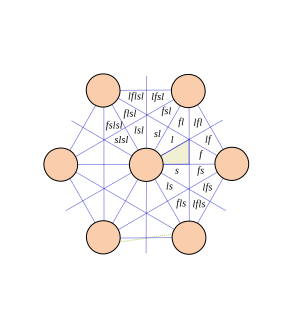
\includegraphics[width=0.45\textwidth]{7diskFundDtiles}
\end{center}
\caption{
(a) The three generators of tiling of the plane by a fundamental domain:
two generators of \Dn{12} tiling, reflection $s$ across the short
disk-disk separation, reflection  $\ell$  across the long disk-disk
separation;
and
a translation generator $f$ that pivots (`flips') a disk center to disk
center by flip across the symmetry line normal to the short disk-disk
separation.
(5) Tiling of the 7-disk by copies of the fundamental domain, labelled
by a (not unique) sequence of the three generators
$\{s,\ell,f\}$, chosen so that each sequence contain one and only on
    disk-to-disk pivot $f$.
        }
\label{7diskFundDflipsA}
\end{figure}
%%%%%%%%%%%%%%\item[Figure 4]%%%%%%%%%%%%%%%%%%%%%%%%%%%%%%%%%%%%%%%%%%

% \item[2014-06-02, 2014-06-08 Predrag]
\refFig{7diskFundDflipsA}\,(a) illustrates the three generators
\beq
    \{s,\ell,f\}
\,.
\ee{c-3gener}
In the international
crystallographic notation, our hexagonal lattice is called $p6mm$,
with point group $6mm$,
where
prefix $p$ indicates that the unit cell is primitive (not centered),
\beq
\Group = \{
e, C_6^+, C_6^-, C_3^+, C_3^-, C_2,
\sigma_{d1}, \sigma_{d2}, \sigma_{d3},
\sigma_{v1},\sigma_{v2}, \sigma_{v3}
\}
\,,
\ee{D12generatorsA}
with $s=\sigma_{d}$ the reflection across the
short disk-disk separation, and $\ell=\sigma_{v}$ reflection across the
long disk-disk separation generators of \Dn{12}. The entire space group
is then generated by adding a disk-to-disk generator $f$ that pivots a
disk center to disk center by flip across the symmetry line normal to the
short disk-disk separation.
We find it convenient to define $C$ as the generator of cyclic rotations
by $\pi/3$,
\[
\ell s = C_6^- = C
\,,\quad
C^6 = e
\,;\qquad
s \ell =  C_6^+
\,,\qquad
s  =  C_6^+ \ell
\,.
\]
There are two short paths from disk to disk: $f$, which keeps the sense
of orientation, and $sf=fs$ which changes it.

\begin{figure}
\includegraphics[width=\textwidth]{7diskFUndDtilesEquiv}
\caption{Shortest equivalent sequences.}
\label{fig:symbolEquivA}
\end{figure}


The (hopefully complete) list of the
equivalence relations, \ie, different sequences of operations reaching
the same copy of the fundamental domain is:
\beq
s s = e
\,,\quad
\ell \ell = e
\,,\quad
f f = e
\,,\quad
C^6 = e
\,;\qquad
f s = s f
\,,\quad
f \ell f=\ell f \ell
\,.
\ee{3generEquiv}
The two flips $f s = s f$ act at $90^0$ and hence commute.
As shown in \reffig{fig:symbolEquivA}, $f\ell f$ and $\ell f \ell$
map the fundamental domain to the same copy. Finally, $C^6 = e$ ensures
that the tiling is hexagonal.

Our task is to generate all distinct
itineraries from $\{s,\ell,f\}$, by pre-pending a letter to a given sequence.
Repeats of the 3 letters are not allowed (so tree of admissible sequences
is binary), and neither is the sixth repeat of the
rotation $C$. The remaining two equivalence relations we impose by
crossing out any itinerary that contains block $f s$ or block $f\ell f$.
Prohibition of the block $f s$ implies that $s$ is always followed by $\ell$,
\ie, we can replace the $s$ at last position in an itinerary by
$ s \to \ell s = C$,
with $\ell C$ prohibited in the next step.
We start with the three starting letters $\{s,\ell,f\}$, and generate the admissible
itineraries tree as follows:
\bea
&s & \quad\quad \ell \quad\qquad f
    \continue
& C & \quad s \ell, f \ell \qquad s f , \ell f
    \continue
&s C, f C & \quad
    C \ell; s f \ell , \ell f \ell \qquad
        C f ; s \ell f
    \label{3generTree}\\
&C^2; s f C, \ell f C & \quad
    s C \ell, f C \ell; C f \ell ;  s \ell f \ell  \qquad
       s C f, f C f  ; C \ell f
    \continue
&s C^2, f C^2; C f C, s \ell f C  & \quad
    C^2 \ell; s f C \ell , \ell f C \ell ;
            s C f \ell , f C f \ell ;  C \ell f \ell  \qquad
       C^2 f ;  s f C f ,  \ell f C f  ; s C \ell f , f C \ell f
\nnu
\eea
All longer equivalence relations in \reffig{fig:symbolEquivA}
can be reduced to the above primitive ones:
\[
f s \ell = s f \ell
\,,\qquad
      f \ell s \ell f \ell f s
    = f C \ell \ell f C
    = (f C)^2
\]

Treat every itinerary as a cycle, simplify by using cyclic permutations:
\bea
&\cycle{s} & \cycle{\ell} \quad \cycle{f} ;
 \quad \cycle{s \ell} \quad \cycle{s f} \quad \cycle{\ell f} ;
 \quad    \cycle{s \ell f} ;
 \quad  \cycle{s \ell f \ell} ;
 \quad  \cycle{s \ell s   f \ell}
\,.
    \label{3generCycl}
\eea

Is $\cycle{f}$ allowed??? Tingnan is right, need to mark the billiard wall as well?

Here is a list (incomplete) of the fundamental domain fixed points, \ie,
sequences containing at least one $f$ obtained by cyclic repeats of
itineraries in \refeq{3generTree} (see \reffig{7diskFundDflipsA}\,(b)):
\bea
\cycle{f} &=& \cycle{06} \,,\qquad \mbox{shift} = 0
    \continue
\cycle{fs} &=&  \cycle{08} =  \cycle{26} \,,\qquad
\mbox{shift} = \jEigvec[0]-\jEigvec[2]
    \continue
\cycle{f\ell} &=&  \cycle{048} \,,\qquad \mbox{shift} = 0
    \continue
\cycle{f\ell s} &=& \cycle{24}
 \,,\qquad \mbox{shift} = 2\jEigvec[0]-\jEigvec[2]
    \continue
\cycle{f\ell s\ell} &=& \cycle{0\underline{10}8642}
 \,,\qquad \mbox{shift} = 0
    \continue
 \cycle{f s\ell s\ell} &=&  \cycle{???}
 \,,\qquad \mbox{shift} = ?
\,.
\eea
In other words, the 6 fundamental domain symbols are 3 rotations
$\{e,C_6,C_6^2\}$ together with 3 rotations followed by a reflection.

Cycles $\cycle{\ell f\ell}$,
$\cycle{\ell fs\ell}$,
\etc, are not distinct fixed points, because using cyclic symmetry and
$\ell^2 =1$ we have
 $\cycle{\ell f\ell}=\cycle{f}$,
$\cycle{\ell fs\ell}=\cycle{fs}$, \etc.


For practice, let's work out a
few  cycles composed of short flights only.
\refFig{7diskFundDflips2}: conversion of elementary cell \po s $\to$
fundamental domain fixed points for the short 2-cycle, 3-cycle and
6-cycle.
Adding long \po s and \rpo s should result in 11 fundamental domain fixed
points in all, and the 11 letters of alphabet of \refref{LorentzDiff}.

%%%%%%%%%%%%%%\item[Figure ?]%%%%%%%%%%%%%%%%%%%%%%%%%%%%%%%%%%%%%%%%%%
\begin{figure}
\begin{center}
(a)\includegraphics[width=0.43\textwidth]{7diskFundDflips2}
(b)\includegraphics[width=0.43\textwidth]{7diskFundDflips3}
\\
(c)\includegraphics[width=0.43\textwidth]{7diskFundDflips6}
\end{center}
\caption{
(a) Elementary cell short 2-cycle , with multiplicity 3 corresponds to
the fixed pint $f$ in fundamental domain, $\cycle{02}=\cycle{f^2}$;
(b) Elementary cell short clockwise 3-cycle $\cycle{084}$, and
counterclockwise 3-cycle $\cycle{048}$, in
fundamental domain $\cycle{048}=\cycle{(\ell f)^3}$.
(c) Elementary cell short 6-cycle of multiplicity 2, in
fundamental domain $\cycle{0\underline{10}8642}=\cycle{(s\ell f\ell )^6}$.
    }
\label{7diskFundDflips2A}
\end{figure}
%%%%%%%%%%%%%%\item[Figure 4]%%%%%%%%%%%%%%%%%%%%%%%%%%%%%%%%%%%%%%%%%%

This is no new the 2-cycle:
$ \cycle{s \ell f \ell f \ell}
= \cycle{s f \ell f f \ell}
= \cycle{s f}
\neq \cycle{046\underline{10}}$,

There is also 2-cycle $\cycle{0369}$ (once we start including longs).

\begin{figure}
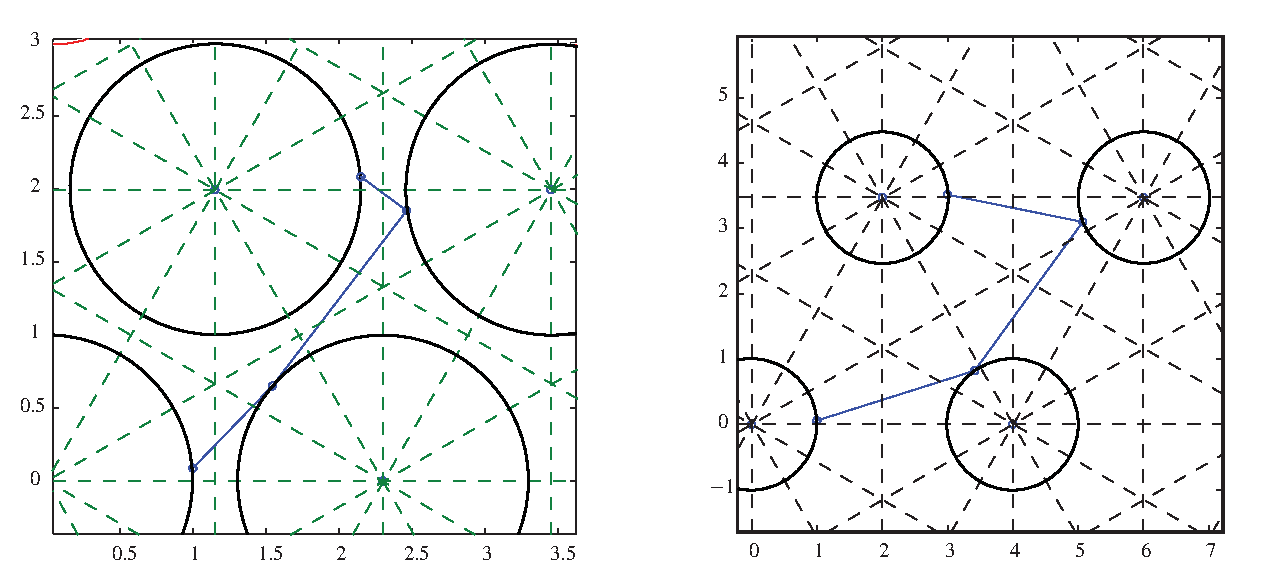
\includegraphics[width=\textwidth]{cycle026.pdf}
\caption{3-cycle \cycle{026} for $w=0.3$ (left) and $w=2$ (right). }
\label{fig:cycle026A}
\end{figure}

% \item[2014-07-11 Tingnan]
I have checked a few cycles and their new symbolic representations. For
example, $\cycle{026}$ and \cycle{0260628}. For cycle $\cycle{026}$ and
$w=0.3$, \reffig{fig:cycle026A}\,(left panel),
the symbolic sequence is $\cycle{f\ell sf\ell f fs}$.
% \item[2014-07-14 Predrag]
Using $f f = 1$
\[
\cycle{f\ell sf\ell f fs}
    = \cycle{f\ell sf\ell s}
    = \cycle{f\ell s}
\,.
\]
For $w=2.0$, \reffig{fig:cycle026A}\,(right panel), the
sequence is slightly different, $f\ell s\ell f \ell fs$, but with the
equivalence relations
% $f \ell f=\ell f \ell$
% \item[2014-07-14 Predrag]
% You are sure that $f\ell f$ equals $\ell f \ell$?
% The have different numbers of flips.
$f s = s f$ and $f \ell f = \ell f \ell$ the end sequence is the
same,
\[
\cycle{f\ell s\ell f \ell fs}
    = \cycle{\ell s\ell f \ell s}
    = \cycle{\ell s f \ell f s}
    = \cycle{\ell s f}
\,.
\]

% \item[2014-07-11 Tingnan]
Similar results can be obtained for $\cycle{0260628}$ in
\reffig{fig:cycle0260628A}.
\[
\cycle{f \ell f s f \ell ...}
\,.
\]
(2014-07-14 Predrag: I give up, let computer do this...)
I have also
checked a few cases when long flights are involved, and the same
conclusion holds: the symbolic sequence we proposed is invariant to
parameter changes.

\begin{figure}
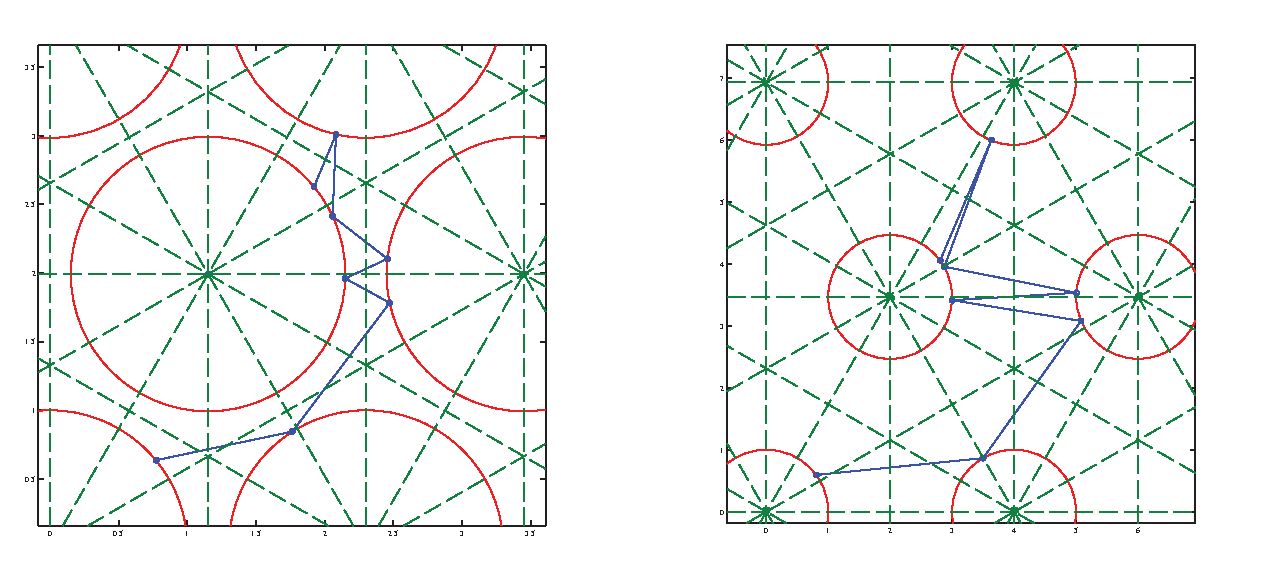
\includegraphics[width=\textwidth]{cycle0260628}
\caption{\label{fig:cycle0260628A}
7-cycle \cycle{0260628} for $w=0.3$ (left) and $w=2$ (right).
}
\end{figure}

\begin{table}
\begin{center}
\begin{tabular}{r}
Symbols and itinerary \\\hline
$\ell$  \\
$s\ell$ \\
$\ell s \ell$ \\
$s \ell s \ell$ \\
$\ell s \ell s \ell$ \\
$s\ell s \ell s \ell$ \\
$s$  \\
$\ell s$ \\
$s \ell s $ \\
$\ell s \ell s$ \\
$s \ell s \ell s$ \\
- \\\hline
\end{tabular}
\end{center}
\caption{All 11 combinations without flip $f$. }
\label{tab:11slcombos}
\end{table}
(2014-07-17 Tingnan) Obervation: since the free flight cannot cross over a disk, the sequence $sl$ or $ls$ can at most appear 3 times, and the $C^6=e$ relation can be re-written as $(s\ell)^3=(\ell s)^3$ (i.e. rotating 180 degree either clockwise or counter clockwise would give the same tile). This also reduces the number of symbols in the state machine(Fig.~\ref{fig:statemachine}). Following the graph, We can generate at most 11 strings without flip $f$(Table ~\ref{tab:11slcombos}). For a single flip, $f$ can be sandwiched by 
any two of the combinations (including the $-$ as a place holder). A valid (and longer) sequence can be generated according to the graph.
\begin{figure}
(a)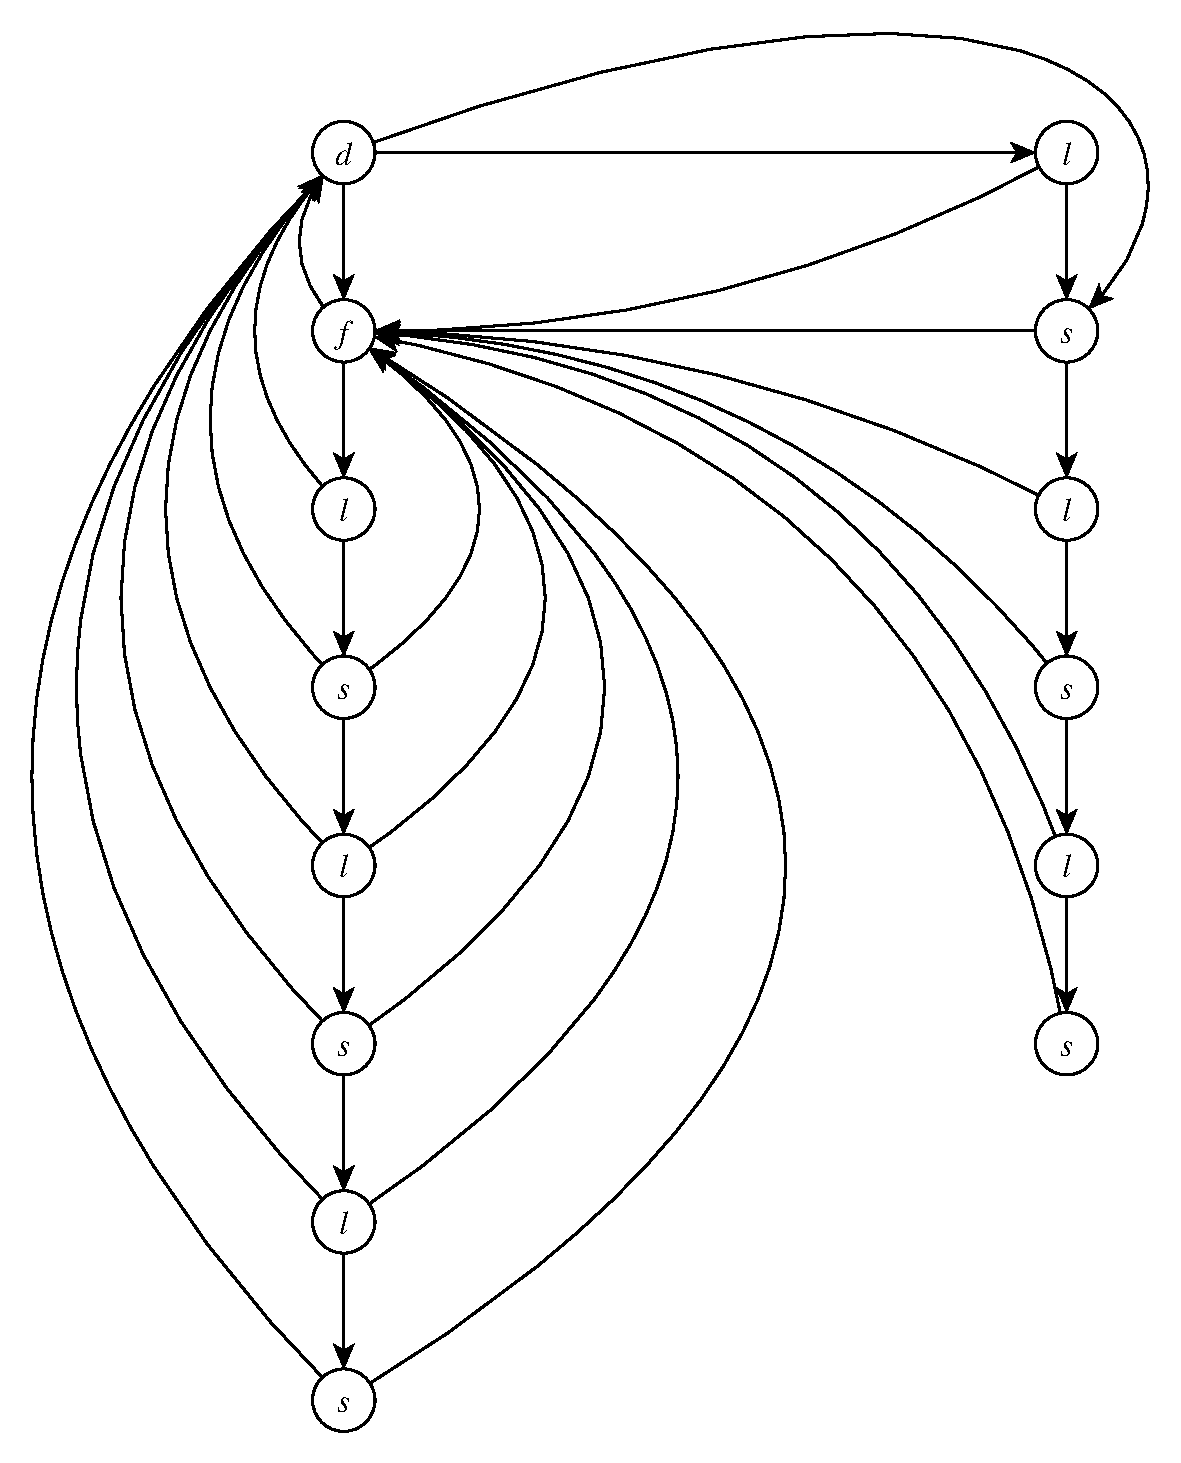
\includegraphics[width=0.5\textwidth]{statemachine.pdf}
(b)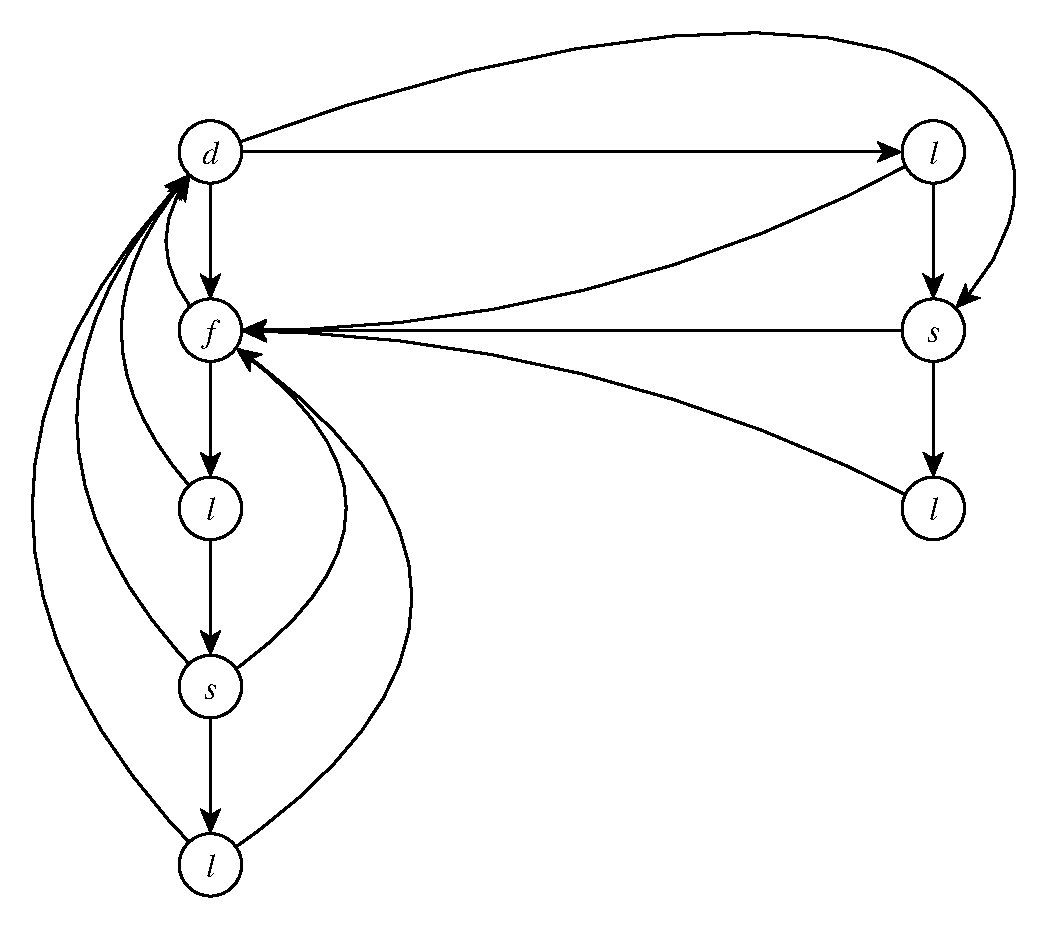
\includegraphics[width=0.5\textwidth]{statemachine_finitehorizon.pdf}
\caption{\label{fig:statemachine} The Markov graph for the symbols.
}
\end{figure}

As soon as the horizon becomes finite the longest free flight without $f$ is $\ell s \ell$. $s \ell s$ is prohibited by the closed horizon. We also have additional pruning rules for a flight between two nearest disks: (A), only one $f$ could appear. (B), $ \ell s \ell $ is forbidden because flight like this cannot hit nearest disk. With those rules we can generate grammatically allowed symbol sequence:

\[
\overbrace{-,\ell,s\ell}\, f\,\overbrace{-,\ell,s,\ell s, s\ell}\, d
\]

There are 12 physically allowed combinations (Tabel~\ref{tab:12symbols}), all of those are labeled in Fig.~\ref{fig:12shortflight}.
\begin{table}
\begin{center}
\begin{tabular}{c|r|c}
\# & Itinerary & corresponding cycle\\\hline
0&$fd$ & \cycle{06} \\
1&$\ell fd$ & \cycle{048} \\
2&$s\ell fd$ & \cycle{24} \\
3&$f\ell d$  & time reversal of $\ell fd$\\
4&$\ell f\ell d$ & ? \\
5&$s\ell f\ell d$ & \cycle{0\underline{10}8642}\\
6&$fsd$  & ? \\
7&$\ell fsd$ & \cycle{26} \\
8&$fs\ell d$ & time reversal of $\ell fsd$ (notice all $fs$ is replaced by $sf$)\\
9&$f\ell sd$  & time reversal of $s\ell fd$\\
10&$\ell f\ell sd$ & time reversal of $s\ell f\ell d$ \\
11&$s\ell f\ell sd$ & ? \\
\hline
\end{tabular}
\end{center}
\caption{All 12 combinations to visit nearest disk(s). }
\label{tab:12symbols}
\end{table}
\begin{figure}
\includegraphics[width=0.5\textwidth]{12shortflight.pdf}
\caption{\label{fig:12shortflight} 12 possible short flights when horizon is finite.
}
\end{figure}

\svnkwsave{$RepoFile: froehlich/dailyBlog.tex $}
\svnidlong {$HeadURL: svn://zero.physics.gatech.edu/froehlich/blog/dailyBlog.tex $}
{$LastChangedDate: 2009-11-21 20:25:56 -0500 (Sat, 21 Nov 2009) $}
{$LastChangedRevision: 29 $} {$LastChangedBy: froehlich $}
\svnid{$Id: dailyBlog.tex 29 2009-11-22 01:25:56Z froehlich $}


\chapter{Research blog on symmetry reduction}
\label{chap:blog}

$\footnotemark\footnotetext{{\tt \svnkw{RepoFile}}, rev. \svnfilerev:
 last edit by \svnFullAuthor{\svnfileauthor},
 \svnfilemonth/\svnfileday/\svnfileyear}$

% J Hightower - former texas politician, author, speaker 1943-
\begin{bartlett}{
Only dead fish go with the flow}
\bauthor{
\HREF{http://www.brainyquote.com/quotes/authors/j/jim_hightower.html}
     {J Hightower}, Texas politician}
\end{bartlett}


\begin{description}
\item[2010/05/10 SF] Definition (9.9) of \emph{stabilizer}
in ChaosBook.org version13, \HREF{http://chaosbook.org/version13/chapters/discrete.pdf}
{Chapter 9 - World in a mirror} seems wrong.

\item[2010/05/10 PC] You are right - we have now
\HREF{http://www.flickr.com/photos/birdtracks/4259634492/}
{replaced ``stabilizer''} by $G_p$-\emph{symmetric} throughout the next chapter.
Please alert me to its occurrences in this chapter, suggest how to
fix them.

BTW, I referenced equation number in your remark with respect to
the stable ChaosBook.org version13 in order that it always links
 correctly: equation numbers etc. keep changing in the unstable,
 currently edited version.


\item[2010/05/11 SF] I started reading chapter 10 on my own.
I do not feel like I have a good grasp of Lie groups and algebras,
do you have any suggestions on what I should read to learn more
or is it not important for the research?.

\item[2010/05/12 PC] En attendant Godot (by the time KGB geniuses have
 your computer configured, the summer might be over), so I moved the
 computer that you were using on Monday to your desk for this summer.

As far as Lie groups and algebras are concerned, ignore them from now - lets
just understand what $SO(2) / U(1)$ invariance does to complex Lorenz equations.
Physicists usually learn $SOn{3}$ next and not the general theory of Lie groups, so lets
start small: invariance on a circle.

\item[2010/05/13 SF] I finished looking through chapters 9 and 10 and the paper. I am going to start looking at the problems from chapter 10 to make sure I understood the material. If any of the problems give me trouble or I'm not sure of the solution I'll post it here.

\item[2010-05-13 PC] That's good, but work within
siminos/froehlich/exerFlow.tex in your blog. Most of the exercises are
already there. Edit them as you see fit, add new ones and their solutions
 if you find that there are missing steps that you need to do in order
to simulate/analyze \cLe.

\item[2010-05-13 PC] You might want to join
\HREF{http://www.zotero.org/groups/cns}
{http://www.zotero.org/groups/cns}
in order to be able to access the papers we are saving there. Nothing
urgent, for now. Search for zotero in siminos/blog/blog.pdf to find
a bit more info about it.

\item[2010/05/24] I started thinking about the problem of when the group tangent at the point is perpendicular to the group tangent at the slice point. I think I understand what is happening but would like you to check my work to make sure I actually do.

    For the $x_1 = 0$ slice for the \cLe\ I think I can show that it is only possible for a trajectory to touch the slice instantaneously unless it is an equilibrium solution: Suppose a trajectory stays in the slice for some interval of time, this means $x_1 = \dot x_1 = 0$ in this interval, which gives us that $y_1 = 0$ during this time. So $y_1$ is constant for some interval of time, so $\dot y_1=0$ here also. Looking at $\dot y_1 = 0$ when $x_1=y_1 =0$ gives $x_2 = -(e/\rho_2)y_2$. Plugging these three restrictions into the equations for $\dot x_2$ and $\dot y_2$ yield the equations $\dot y_2=-\sigma y_2 (1+(\rho_2 / e))$ and $\dot y_2 = (\rho_1 - z)(-e/\rho_2)y_2-y_2$ this means that $-\sigma y_2 (1+(\rho_2 / e))=(\rho_1 - z)(-e/\rho_2)y_2-y_2$ provided $y_2$ is nonzero, then $-\sigma (1+(\rho_2 / e))=(\rho_1-z)(-e/\rho_2)-1$. z is the only variable in that equation, so it must be constant. This means that $\dot z = -b z + x_2 y_2 + x_1 y_1=-b z+ (-e/\rho_2)y_2^2=0$. Again $y_2$ is the only variable so it too must be constant, so $x_2$ is also constant. This means the solution can stay in the slice only if all its values are constant, so it is an equilibrium solution. There are possibly some divide by zero difficulties, but hopefully a similar argument will hold for these cases.

    So we do not run into this problem for the \cLf.

    As I understand it, the reason the group tangent along the trajectory being perpendicular to the group tangent of the slice causes problem is because this means that doing an infinitesimal rotation at the point keeps it inside the slice so the point is not a unique representative (at least when doing the infinitesimal rotations), is this correct?

    When choosing the slice to be a hyperplane through a point, it doesn't have to be perpendicular to the group tangent at some point does it? As long as the group tangent at any point isn't contained inside the hyperplane there shouldn't be a problem locally.

    I thought about trying to show that this condition being true for an interval of time implies it is always true and I have no clue how to go about it so far. I think I see why it is true if the ODE is linear like in QM, but my argument is not quite complete.


\item[2010-05-25 ES] Linear slices are indeed not flow invariant, so only equilibria (or any points in $\Fix{\SOn{2}}$) stay on the linear slice
under equivariant dynamics. Another way to show this would be

\exercise{Linear slices are not flow invariant}{\label{exer:SliceInvCLf}
(a) By forming the inner product of the group tangent direction with the velocity field of \cLe\ show that the linear slice $x_1=0$ is not invariant under \cLf.
(b) Can we construct a flow invariant linear slice? (c) Repeat the exercise using as less information as possible about \cLe.
\authorES{2010-05-25}
}
\solution{exer:SliceInvCLf}{Linear slices are not flow invariant}{(a) The inner product is eq. (71) in internal version of my thesis, in case you need to double check your result. The rest is left to you. (c) Predrag finds such warnings useless, but I have not tried to solve this part. You have of course to make use of equivariance
and perharps of the group representation. Flow contraction of \cLf\ might come in handy, too.
}

The trouble is that \refexer{exer:SliceInvCLf}, or what you have shown above does not help us, I think, to conclude that the singularity at $x_1=x_2=0$ is not reached by the dynamics. What would help, would be

\exercise{$x=0$ singularity in \cLf}{\label{exer:SingOnFixedspCLf}
(a) Show that for \cLf\ $x_1=x_2=0$ implies that $y_1=y_2=0$, that is we can only run into $x_1=0$ slice singularity in $\Fix{\SOn{2}}$ (the $z$ axis).
Since $\Fix{\SOn{2}}$ is flow invariant, general dynamics cannot reach it and we can safely apply the method of moving frames/slices. (b) Is this
result \cLf\ or group representation specific? Can you prove it using as less information for \cLf\ as possible?
\authorES{2010-05-25}
}
\solution{exer:SingOnFixedspCLf}{$x=0$ singularity in \cLf}{Sadly, I do not know how to solve this.}

Note that one might be even more lucky than \refexer{exer:SingOnFixedspCLf} suggests and be able to show that we can only run into a singularity at the origin.

\item[2010-05-28 ES] I am sure you've noticed that when you try to integrate in invariant polynomials basis
you run to some singularity - I had never tried that before. I've only looked at your Mathematica files,
do you get the same behaviour with Matlab as well? I've tried playing a bit with the integrator,
for instance using implicit Runge-Kutta should work if stifness and not a singularity was the problem.
Any intuition on what happens and why? If you have access to Gilmore and Letellier book\rf{GL-Gil07b},
the section \emph{Tips for Integration} might be helpful.

\item[2010-05-28 PC] We have the book in
\wwwcb{/tutorials}.

\end{description}



\end{document}
